\documentclass[../dejiny-rodu-prusiku.tex]{subfiles}

\begin{document}

% str 91 @ 107
\section{Odnož Výrov II - větve Výrov}

Potomci Václava Prusíka, sedláka z Výrova

1822-1892

Sedmým dítětem Vojtěcha Prusíka, rychtáře ve Výrově, který sem přišel v r. 1803 ze Sedlce, byl syn Václav. Narodil se ještě v dobách roboty 7. 9. 1822  ve Výrově č. 18. Usedlosti, kde se narodil, říkalo se od pradávna "u Boudů" a jeho matka Anna, roz. Fenclová, byla také potomkem prvního Boudy, který v roce 1610 se ujal hospodařeni na tomto statku.

Václav Prusík, ačkoliv neměl příležitosti navštěvovati vyšší školy, přece jen nabyl dosti značného vzdělání. Četl hospodářské listy, odborné knihy i mnoho jiného poučného, co mu jeho bratr vikář Blažej z Prahy posílal. Když jeho otec Vojtěch zemřel v roce 1841, stal se mu poručníkem jeho švagr Vojtěch Karez z Horní Břízy. Brzy však se oženil. Našel si nevěstu v městečku Kozojedech. Byla to Josefa Kotasova z tamní usedlosti č. 35, narozená 20. 9. 1826. Její otec Martin Kotas narodil se 18. 10. 1795 a zemřel na výměnku u své dcery ve Výrově 12. 7. 1879. V té době totiž statek v Kozojedech už Kotasům nepatřil. Byl jíž předtím silně zadlužen a prodán manželům Smolíkovým, ale v roce 1889 opět se tam dostal člen našeho rodu, Václav Prusík z Hodyně. Také matka Josefy, Marie Kotasová zemřela ve Výrově. Narodila se jako Píplová v Kozojedech 29. 1. 1802 a zemřela 22. 2. 1882. Ve svatební smlouvě z 28. ledna 1843 mezi Václavem Prusíkem a Josefou Kotasovou je tato úvodní věta, jejíž duch se pak opravdu v životě novomanželů zcela naplnil: „Slibujou sobě nastávající manželé Václav Prusík a Jozefa Kottas až do smrti věrnou a upřímnou lásku.“ Za dva dny po této svatební smlouvě, uzavřené na Metternichově panství v Plasích, oženil se Václav Prusík s Josefou Kotasovou. Stalo se to 30. ledna 1843.

Ještě před rokem 1848, kdy byla zrušena robota a nastalo jiné politické uspořádání v obcích i okrese, byl Václav Prusík rychtářem ve Výrově. Tak jako před ním jeho otec Vojtěch Prusík a předchůdci. Na statku "u Boudů" bývala od pradávna rychta, jak jsme to vylíčili již na straně 20. Od roku 1850, když byl utvořen okres Kralovice a v obcích byli starostové již voleni a ne jak předtím, rychtáři jmenováni, stal se Václav Prusík prvním voleným starostou Výrova. Byl jim až do smrti a po něm i syn Vojtěch až do roku 1912, kdy statek prodal.

Václav Prusík se svou ženou Josefou měli jedenáct dětí. Byli to: Nejstarší syn Blažej, narozený 1. 1. 1844. Stal se profesorem filologie, hlavním jeho působištěm byly Klatovy a zemřel 15. 10. 1912 v Praze. Druhý byl syn František narozený 24. 11. 1845. Také on se stal profesorem filologie, v níž zvláště proslul a zemřel 7. 6. 1905 ve Stupčicích u Tábora. Třetím dítětem byla dcera Josefa. Narodila se 28. 2. 1848, provdala se za sedláka Matěje Urbánka do Lednice, kde zemřela 28. dubna 1924. Druhá dcera
% str 92 @ 108
byla Marie, narozená 29. 7. 1851. Provdala se za sedláka Josefa Koukla do Bílova, kde zemřela 6. 2. 1908. Třetím synem byl Václav Prusík narozeny 2. 1. 1854. Stal se magistrátním úředníkem v Praze, kde zemřel 16. 9. 1915. Šestým dítětem byl syn Vojtěch narozený 3. 4. 1856, převzal po otci rodný grunt, který však v roce 1912 prodal a zemřel u své dcery ve zněmčené obci Kolešovicích 15. 3. 1920. Třetí dcerou byla Anna. Narodila se 15. 12. 1858, provdala se za Josefa Kouru, sedláka v Bílově, kde zemřela 14. 12. 1935. P0 ní se narodila dcera Veronika 24. 11. 1861. Byla provdána za rolníka Josefa Valentu ve Výrově a tam zemřela 5. 11. 1936. Pak se narodil syn Josef 27. 2. 1863. Byl celním úředníkem a zemřel 8. 8. 1940 v Praze. Poslední dcerou byla Barbora narozené 27. 11. 1865, provdaná za živnostníka Waltera v Klatovech, kde zemřela jako nejstarší ze všech sourozenců 29. 5. 1958. Poslední byl syn Antonín, narozený 19. 2. 1869. Byl nejmladší a  nejdříve zemřel. Původně byl u finanční stráže, krátce jako ženatý měl živnost v Příbrami, kde zemřel 16. 4. 1899.

Byla to tedy neobyčejně četná rodina a starostí více než dost. Jistě by to bývalo způsobilo rozpadnutí statku, kdyby se nebyl vyskytl zachránce v nejstarším sou­rozenci. Byl to Blažej Prusík. Ten v době, kdy se posílali hoši na studie, byl již vikářem metropolitního chrá­mu sv. Víta v Praze. Tento kněz uvolil se některé hochy, své synovce, přijmouti do svého opatrování ve studiích. A tak čtyři synové odešli z domova a vystudovali v Praze. Byli to Blažej, František, Václav a Josef. Poslední Antonín vystudoval alespoň částečně v Klatovech a hospodářství zůstalo synu Vojtěchovi.

Václav Prusík byl na svou dobu velmi pokrokovým hospo­dářem. Nepomohly mu k tomu jenom odborné spisy, které pilně četl, ale také cenné rady jeho pražského bratra Blažeje. Václav Prusík byl prvním zemědělcem ve Výrově a širokém okolí, který začal sekati obilí kosou místo srpem. Již za jeho života vysadilo se ve Výrově mnoho ovocného stromoví, uváděly se v život nové hospodářské stroje. Nepůsobil však tento sedlák jen blahodárně v obci, ale i v okrese, neboť byl také dosti dlouho členem okresního výboru v Kralovicích. Mnoho jeho dobrých nápadů se uskutečnilo.

Velké neštěstí Václava Prusíka stihlo, když zemřela ve svých jednapadesáti letech jeho žena Josefa. Bylo to 25. 5. 1877. V té době jeho syn Vojtěch byl na vojně a všechna tíha starostí o rodinu a hospodářství ležela jenom na něm. Jeho dopisy, které se zachovaly, svědčí o lásce k rodičům a celé jeho rodině a také k celému širokému okolí.

Krásný je na příklad jeho dopis o smrti maminky Anny Prusíkové roz. Fenclové. Narodila se ješě za panování císaře Josefa  II. V roce 1785 a zemřela 6. ledna 1859. Opravdu vážně churavěla jen dva dny. Dopis ze 16. ledna 1859, adresovaný jeho bratru vikáři Blažejovi do Prahy, začíná
% str 93 @ 109
takto:

„Nejmilejší pane bratře!

Oznámil jsem Vám předešle v krátkosti zprávu zajisté neočekávanou, totiž čas úmrtí drahé matičky naší, připověděl jsem pak Vám, že Vám budoucně obšírněji psáti o tom budu, poněvadž více času k tomu jsem neměl, jelikož jsem chtěl sám tímto krátkým listem jenom v známost uvésti, kdy a který den pohřeb naší drahé matičky provázeti budeme a protož  Vám to musím tehdy obšírně vypsati, neboť mé jaksi neobyčejně truchlivé a smutné srdce ustavičně k tomu nabízí, abych Vám o tom co nejrychleji zprávu dal, snad doufá ve Vás, jakožto nejvěrnějším a nejúpřímnějším příteli po Bohu na tomto světě polehčení dojíti a protož slyšte:

Bylo to právě dne 5. ledna ráno, když jsem naši milou matku, ze sedničky do naší sednice jak to obyčejně bývalo, odvedl a usadil a na něco neobyčejného já ani ona ani žádní jiní, nepomysliv, ubíral jsem se zase, jako obyčejně po prácech svých a ona pak ještě sama mně pravila, abych jenom po práci šel, že se ještě nějakou chvíli modliti bude. Na to já odešel. Přijdu pak po nějaké chvíli opět do sednice a ona seděla u kamen. Manželka má jí předložila snídani a ona se ještě s tím naším nejmenším chlapcem Vojtěchem nasnídala a vyrážela, neboť ten byl její největší miláček. A tak toho nejmenšího zlého znáti na sobě nedala.“

V dopise dále líčí Václav Prusík krátký průběh nemoci své maminky a její smrt, která nastala druhého dne. Píše dále o pohřbu a líčí svou tesknotu, když zůstal po odjezdu svých sourozenců a přátel samoten a vzpomíná na svou zemřelou matku těmito slovy: „A tak odebrav se zase zpátky do města tam pak všechny přátele a známé a sousedy dle obyčejného pořádku slušně poctiv, konečně s bratřími a sestrami svými domů se odebrav, kdežto oni ještě přes dvě noce u nás pobyvše konečně domů se odebrali a takto zůstav opět samoten, doma velice teskliv a truchliv jsem byl. Při každém pohlédnutí na místo, na kterém drahá matička naše sedá­vala, vždy jakoby mě do srdce bodnulo a říkalo ach, drahá matičko má, kéž by si zde ještě byla...“ A tak šel-li jsem do chléva nebo do stodoly neb na pole, všude se mnou stanula, jak z úrody radost mívala a o vše se nejlépe starala. Kdybych s Vámi, pane bratře, mluviti mohl s Vám zde všechnu tu mou bolest vypověděti mohl. S tím uzavírám a končím list můj, Vás srdečně ode  všech zde bydlících i přátel uctivě pozdravuji a líbám a dobrého zdraví přeju.“

Václav Prusík, otec jedenácti dětí ještě za svého života krom nejmladší dcery Barbory, provdal dobře všechny ostatní. Velikou starost měl také o to, aby dobře vystudovali jeho synové a našli si slušnou životní existenci. Zemřel na výměnku na tzv. zauzlení střev 11. 2. 1892 ve Výrově. Ve svém mladém věku zažil ještě robotu i zaostalejší hospodaření na venkově, na konci života viděl již rychlý vzestup našeho národa a nové modernější hospodaření. Svým životem a dílem k tomu všemu vydatné přispěl.

% str 94 @ 110
Prvním dítětem Václava Prusíka a jeho ženy Josefy, roz. Kotasové ve Výrově byl syn Blažej. Narodil se 1. 1. 1844. Byl druhým synovcem vikáře Blažeje Prusíka v Praze, který k němu přišel do Prahy a s jeho pomocí vystudoval. Blažej Prusík studoval na pražském staroměstském akade­mickém gymnasiu od roku 1855 až do roku 1863. Pak stu­doval na filosofické fakultě Karlovy university a s těmito studiemi byl právě hotov v době prusko-rakouské války v r. 1866. Tehdy se nesnadno cestovalo z Kralovicka do Prahy a jak to bývalo, na to vzpomíná velmi výstižné Blažej Prusík.

\subsection{Jak cestovali studenti}

"Než se začalo jezdit po dráze z Rynholce do Brusky v Praze, a to bylo až od roku 1861, jezdili jsme z domova do Prahy a odtud domů s formany nebo i chodili pěšky. Než jsme se dostali ze Strahovské brány nebo zase do ní, museli jsme míti pas. Domů jsme se dostali jen jednou v roce a to po vysvědčení začátkem srpna. Jindy jsme do­mů nemohli, neboť mezi svátky bylo prázdno krátké. Planuli jsme touhou po domově právě proto také. že celý rok jsme se domů nedostali. Rodiče jsme viděli o svatém Janě, kdy do Prahy jezdívali. Protože jsme bydlili na Hradčanech na Vikárce, jakmile jsme přinesli vysvědčení, šli jsme hned na Pohořelec hledat tamnější četné zájezdní hospody, kde bychom našli nějaký povoz, jedoucí směrem k Rakovníku. Stávaly tam totiž fůry, které do Prahy přivezly obilí nebo něco jiného. Ranečky jsme měli malé, jen nějaké nejnutnější jídlo. Často jsme zmokli v Rakovnickém lese na kůži a když to nešlo s povozem šli jsme pěšky. Velmi často jsme přišli domů s odřeninami a pryskýři na nohou. Milosrdná hostinská leckde, když jsme promokli, půjčila nám něco suchého šatstva a naše sušila na velkých kamnech v šenkovně. Trvalo to někdy hezky dlouho než uschlo, obloha se vyjasnila a mohli jsme se vydat na další cestu k domovu. Jednu výhodu však takové cestování mělo. Bylo levné.

Cestování dostavníkem bylo již veselejší. Za městem dali se koně do mírného klusu, ale to netrvalo dlouho. Vždyť  jeden pár koní musel vydržet na celou cestu. Proto když začala silnice stoupat, kočí slezl z kozlíku a brzy volal do vozu: „Prosím, pánové vystoupnou, tady to jde do vrchu!“ a tak'jsme nejen sesedli, nýbrž i podle svých sil zatlačili, aby se mohlo jeti dále. Někdy v dostav­níku byla dobrá společnost, jindy zase nebyli spolucestující příjemní.

Nesmírně významná událost nastala pro nás v roce 1861, když koňská dráha z nádraží  Brusce začala také vozit pasažéry. Byla zřízena v roce 1836 až do Lán, odkud vozila výhradně dříví z křivoklátských lesů  do Prahy. Teprve v roce 1861 se zrodila šťastná myšlenka voziti také osoby ve zvláštních vozech, omnibusu podobných i se sedadly na střeše. Poslední stanice byl Rynholec. Směrem od Prahy bývali do vozu zapřaženi dva koně za sebou, ku Praze stačil jeden. Nakonec se naše dráha i bez toho jednoho koně obešla. Když jsme totiž dorazili na stanici
% str 95 @ 111
„U černého koníčka", která byla za Jenčem 15 km od Strahova, tu se kůň vypřáhl a vůz přirozeným svahem ujížděl ku Praze. Kdykoliv jsme se přiblížili ke stanici, konduktér zabrzdil, vůz se zastavil, pasažéři se vystřídali, načež zřízenci vůz strčili a ten uháněl vesele dále, až na poslední stanici v Brusce zůstal stát."

Takto cestovali ve svých studentských letech Jan a Tomáš Prusík do Horní Břízy, Blažej a František Prusík do Vý­rova. Později pro ostatní to už bylo snazší.

Blažej Prusík po skončených studiích na universitě stal se suplentem na českých paralelkách při německém gymna­siu premonstrátském v Plzni a to v letech 1866 až 1871. Od 1. 10. 1871 stal se profesorem na gymnasiu v Klatovech a zde působil 34 let. Neomezoval se jen na učitelskou činnost, ale byl i veřejně činný. Jeden čas byl dokonce předsedou pěti spolků a sám vzpomíná, že by mnohem raději byl seděl v každém spolku jakožto prostý člen. Předsedal Literární jednotě, Zpěváckému spolku Šumavan, Hasičskému sboru, Právovárnému měšťanskému pivovaru a Bruslařskému klubu. Z tohoto klubu vytvořil se v pozdějších letech SK Klatovy. Jeden čas byl Blažej Prusík i předsedou Okrašlovacího spolku. Také byl členem obecního a okresního zastupitelstva v Klatovech.

Blažej Prusík patřil mezi spravedlivé, ale velmi přísné profesory. Mezi jeho žáky byl i pozdější slavný lékař Thomayer nebo i básník Jaroslav Vrchlický. Na jeho činnost vzpomíná ve svém románu "Osení" spisovatel Hais-Týnecký. V tomto díle líčí spisovatel život v Klatovech v minu­lém století a také klatovské studie Jaroslava Vrchlického (Emila Frídy). Píše: "Na latinu, řečtinu a němčinu dostali po Hylmanovi profesora Blažeje Prusíka. Přišel do Klatov z Plzně a stal se jejich třídním, který je měl dovésti až k maturitě. Byl to tuze krásný člověk, vysoký, štíhlý s černým plnovousem. Nikdy se nerozčílil, ale byl velmi přísný. Přišel, zasedl ke katedře, a již se neodtrhl. A jako on, také oni (žáci) seděli v lavicích a odpovídali, když je vyvolával a četli Platona, Sofokla a Horáce. Neklidného ducha Vrchlického tato Prusíková metoda příliš nebavila."

Když Šmilovský, který byl v těch dobách také profesorem na gymnasiu v Klatovech, napsal svého "Krupaře Kleofáše" podle občana Junga, sběratele starožitností v Klatovech, rozbírali toto dílo studenti poprvé v Prusíkové třídě. Mnoho je vzpomínek na klatovské profesorování Blažeje Prusíka.

Již v Plzni, kde byl Blažej suplentem, poznal svou nastávající družku života Emilii roz. Holou ze Štěpánovic u Klatov. Byla to dcera nájemce tamního Černínského dvora, kde se narodila 10. 4. 1859. - Blažej s Emilií měli svatbu 11. 5. 1881. Z tohoto manželství narodili se syn Bohumil a dcera Blažena, kteří dospěli. Dcera Marie zemřela jako pětiletá v roce 1893 na spálu.

% str 96 @ 112
Blažej Prusík byl také jeden čas redaktorem, Klatovských listů, při jejichž založení byl kmotrem. Za přispění své ženy musil však obstarávat jeden čas i expedici listu a celá tato redaktorská činnost ho stála sto zlatých. Blažej sebral také velké množství písní, které slýchával na poli, také při česání chmele a o obžínkách. Bylo to z kraje Plzeňského, Klatovského, Domažlického, ale i Píseckého, Táborského a Budějovického. Měl také četnou sbírku lidových jmen pozemkových to jest jak se lidově říkalo některým parcelám polí a luk. Tak na příklad u gruntu Prusíků v Sedlci jmenovala se některá pole a louky takto: na vršíčku, skalice, jezera, za humny, baba, zahrádka, na velkým, za luhem, u jámy,  pruchlavice, kamenej, paseka, nebo u luk, na psinách, hranice, za luhem, za poustkou, palouk, mezi jamama, předeství atd.

V létě 1905 odešel Blažej Prusík do pense a protože jeho syn vstoupil ten rok na universitu, kde začal studovat medicínu, odstěhoval se s celou rodinou do Prahy. Zde působil ještě nějaký čas na Vyšším dívčím gymnasiu na Vinohradech. Ve volné chvíli chodil d0 Zemského archivu a shromáždil velmi cenný materiál o naších. předcích, zvláště pokud jde o výrovskou větev. Blažej Prusík zemřel v Praze na Vinohradech 15. 10. 1912 a jeho žena ve stejném dnu a měsíci 15. 10. 1939.

\subsection{Kardiolog světového jména}

Syn Blažeje Prusíka, Bohumil, narodil se v Klatovech 26. 5. 1886. Vystudoval úspěšně klatovské gvmnasium. Jeho spolužáci vzpomínali na něj v dobrém, neboť i když byl premiantem, nezapomínal při vyučování ani na ty, jimž to tak nešlo. Ochotně napovídal a dával opisovat, Měl hudební nadání. Tehdy vytvořili si studenti kapelu, v níž Bohumil byl dirigentem. Jeho přítel Václav Talich, který tehdy studoval také na klatovském gymnasiu, byl jen prostým účinkujícím. Později vyměnili si role. Z Talicha stal se nejslavnější náš dirigent a z Prusíka zase slavný dirigent medicíny. Bohumil studoval v Klatovech i se svým bratrancem Blažejem Prusíkem z Výrova a Blažejem Kouklem z Bílova. Také s ním studoval jeho nevlastní bratranec Vojtěch Walter, syn jeho tety Barbory, provdané v Klatovech. Se svým bratrancem Blažejem Prusíkem byl Bohumil Prusík promován v roce 1910 na doktora medicíny. Již za studií vstoupil na první stupeň fakultního pracovníka jako demonstrátor u slavného zakladatele české pathologické anatomie prof. Jaroslava Hlavy. Po promoci působil na několika klinikách a ještě do začátku první světové války prošel dalšími fakultními hodnostmi u prof. Thomayera.

Již v roce 1912, jako šestadvacetiletý mladý lékař dostal se do Anglie. Tam poznal slavné badatele v oboru srdečních chorob, zejména J. Mackenzieho a Thomase Lewise, u nichž v Londýně pracoval. Odtud také v roce 1912 přivezl první elektrokardiograf do Čech a s ním pak začal na klinice pracovat. Dnes si mladí lékaři sotva uvědomí, co to tehdy znamenalo.

% str 96+1 @ 113
\begin{figure}
\centering
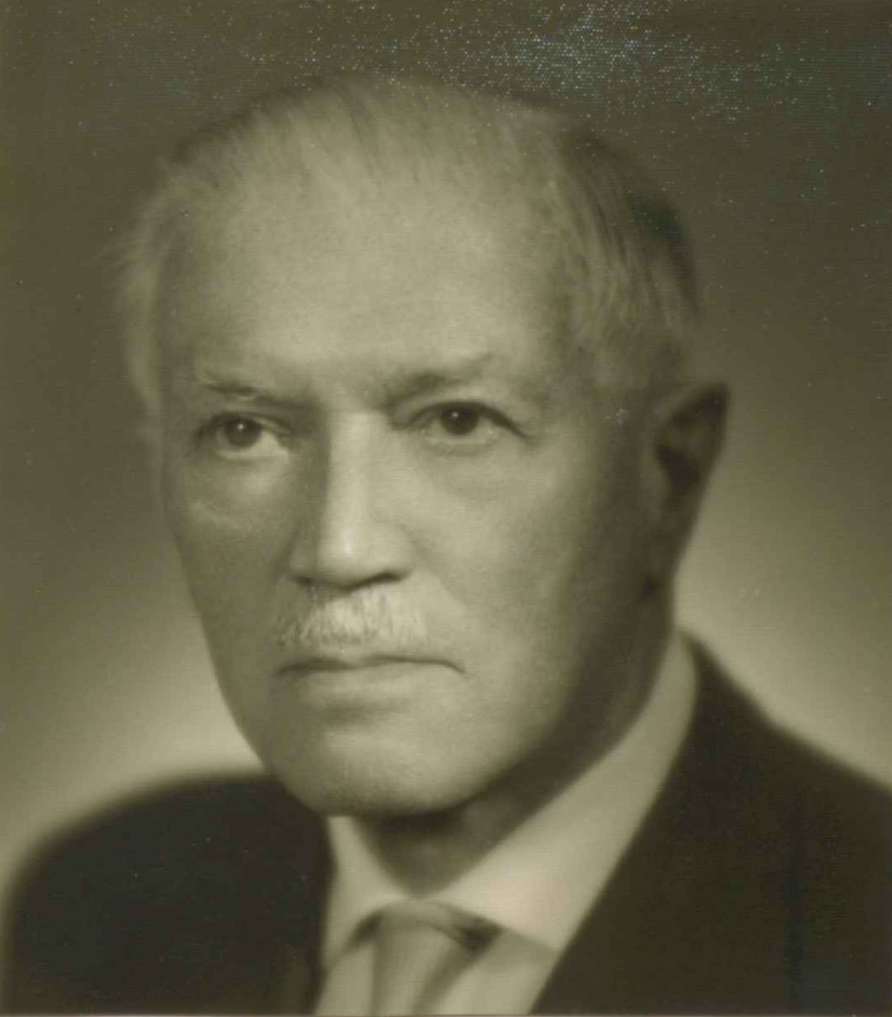
\includegraphics[width=\textwidth, height=\textheight, keepaspectratio]{113-a-prof_mudr_bohumil_prusik}
\caption{Prof. MUDr. Bohumil Prusík, kardiolog světového jména (1886 – 1964)}
\label{fig:113-a-prof_mudr_bohumil_prusik}
\end{figure}

\begin{figure}
\centering
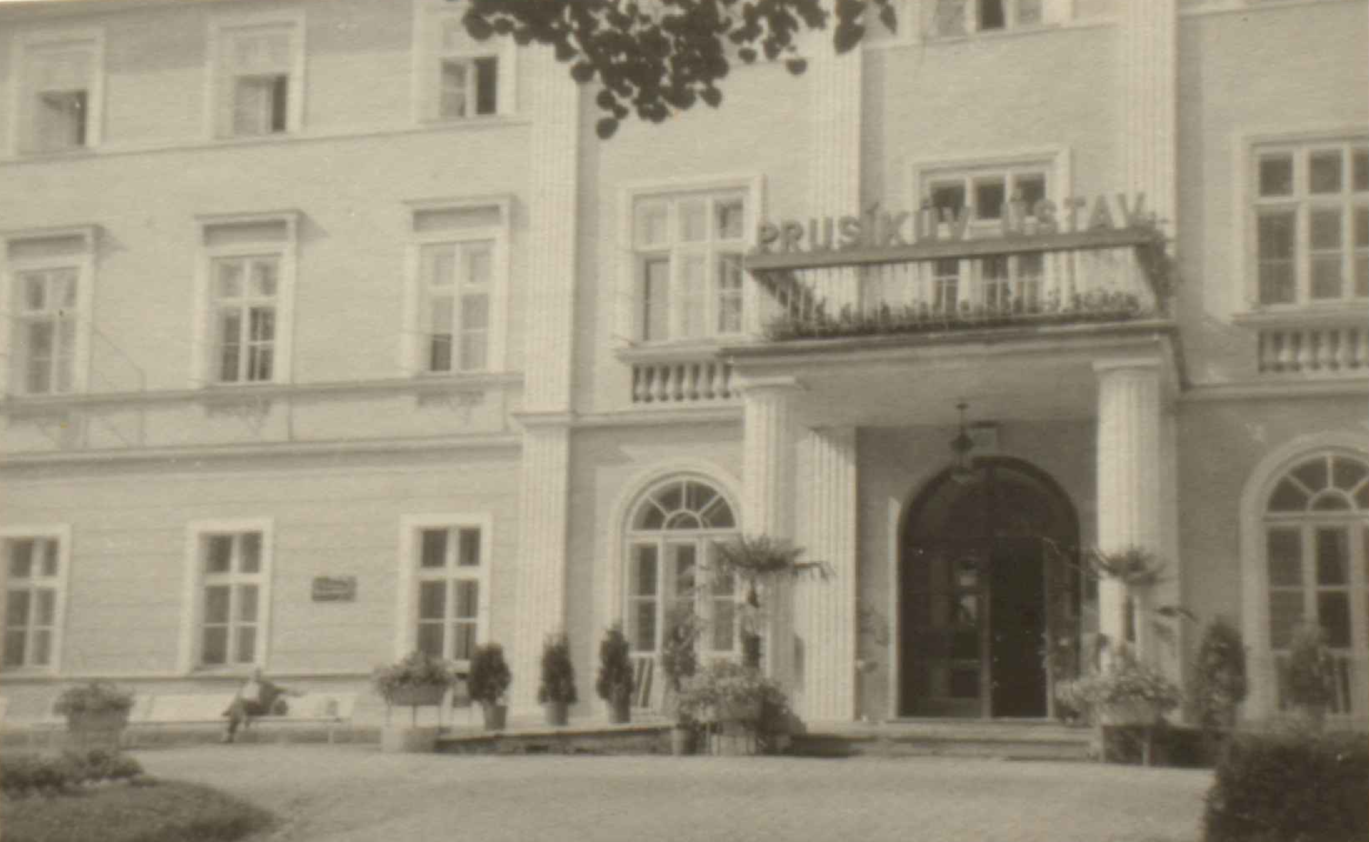
\includegraphics[width=\textwidth, height=\textheight, keepaspectratio]{113-b-prusikuv_ustav}
\caption{Prusíkův ústav v Konstantinových Lázních}
\label{fig:113-b-prusikuv_ustav}
\end{figure}

% str 97 @ 114
V roce 1920 habilitoval se z pathologie a therapie vnitřních nemoci a v roce 1928 stal se mimořádným profesorem Karlovy university. Za pět let nato, v roce  1933 stal se přednostou pro pedeutické kliniky. V roce 1935 byl jmenován řádným profesorem Karlovy university.

Anglický způsob vědecké lékařské práce našel v Bohumilu Prusíkovi nadšeného přívržence a propagátora. Velká řada vědeckých prací, které vydal, týká se srdečních chorob. Jeho vědecká činnost se však zabývala celou internou. Bohumil Prusík měl tolik světových prioritních objevů, že byl navrhován pro Nobelovu cenu. Příchod druhé světové války zmařil však další toto jednání o tom.

Bohumil Prusík u nás první poznal za živa podle křivky elektrokardiografu infarkt myokardu. Dnes je stěží uvě­řitelné, že jsme do té doby tuto diagnosu klinicky u nás neznali. Bohumil Prusík nebyl jen první z našich lékařů, kteří začali za hranice jezdit dále než jen do sousedního Německa, byl také z našich prvních, za kterým začali jezdit vědečtí pracovníci z Francie, Belgie, Holandska i Spojených států a Anglie. Jeho mladší spolupracovník akademik prof. Dr. Josef Char­vát řekl o něm toto: "Chci upozornit, že před více než třiceti lety (řečeno v roce 1964) tušil, kam půjde medicína. Tehdy se stonalo a umíralo hlavně infekcemi. A Prusík pojednou začal intensivně a soustředěně stu­dovat cévy. Vypracoval se na světového vedoucího angiologa (nauka o cévách). Dnes mu vývoj dal za pravdu. Už se neumírá na tyf, záškrt, tolik na tuberkulosu, ale na cévy. Totéž platí i pro další Prusíkův zájem, totiž pro gerontologii. Když se jí začal obírat, soudili někte­ří, že je to podivínství. Dnes je to jeden z hlavních zájmů civilizovaného lidstva. Profesor Prusík byl ozdobou Československé akademie věd. Zanechal dílo, které podstatně usměrnilo náš lékařský vývoj v posledních čtyřiceti letech a které zasáhlo daleko za hra­nice. Zůstane nesmrtelné."

V září 1961 vyvrcholila životní vědecká činnost profesora Bohumila Prusíka čtvrtým mezinárodním kongresem angiologickým v Praze. Stal se presidentem tohoto kongresu a byl po dobu několika let i presidentem mezinárodní unie angiologické se sídlem v Paříži. Prof. Bohumil Prusík byl ovšem také čestným členem velikého množství společností a spolků u nás i v cizině. Jeho vědecké úspě­chy byly uznávány ve světě a když v roce 1967 mluvil o něm v Praze slavný americky vědec prof. White z Harvardské university, prohlásil otevřeně na přednášce v Purkyňově společnosti, že Prusík patří k nejslavnějším kardiologům světa.

S profesorem Whitem, který byl osobním lékařem americké­ho presidenta Eisenhowera, zahajoval Bohumil Prusík v mladých letech svou vědeckou dráhu v Anglii a on také byl nejlepším svědkem dalšího jeho rozletu. Proto mají jeho slova takovou platnost.

% str 98 @ 115
Bohumil Prusík měl nesčetné množství přátel, také v uměleckém světě. Mezi nejbližší přátele patřili umělci zvučných jmen jako byli Talich, malíř a sochař Obrovský, malíř Otakar Nejedlý a další jiní. Po druhé světové válce jezdil téměř každý rok prof. Bohumil Prusík do Mariánských Lázní a tam byl na aktivním odpočinku, vždy v létě tam ordinoval jako host. Bohumil Prusík se oženil za první světové války s Annou Kotlandovou nar. 1. 1. 1891 v Praze. Z tohoto manželství narodil se syn Bohumil. Nebylo však nejšťastnější a bylo před druhou světovou velkou rozloučeno. Jeho sestra Blažena vedla mu pak domácnost v Praze na Vinohradech, Na Valdeku.

Veliký kus života věnoval Bohumil Prusík nemocem srdce a cév a je ironií osudu, že právě tato nemoc ukončila i jeho život. Dlel tehdy opět v létě ve svých milovaných Mariánských Lázních a připravoval se na cestu do Paříže, kde měl působit ve funkci presidenta Mezinárod­ní angiologické unie. Již se tam však nedostal, byl raněn mozkovou mrtvicí 6. 9. 1964. Byla to poslední cesta jeho do Prahy, do níž se tolikrát v životě vracíval ze světa, kde přednášel, studoval a odkud přinášel naší medicíně tolik cenných poznatků. Jeho popel je uložen na vinohradském hřbitově v hrobě jeho rodičů.

Jistě není nadsázkou, že prof. Bohumil Prusík byl jednou z největších ozdob našeho prastarého rodu. Sám k němu také vždy lnul a hrdě se k němu hlásil. Tvrdíme, že profesor Bohumil Prusík byl ozdobou rodu a je tomu skutečně tak. Proč? Kdykoliv a kdokoliv z nás Prusíků se představil nebo představuje, vždy snad se setká s otázkou, zda je spřízněn se slavným lékařem Prusíkem. Tak byl všude znám v naší veřejnosti. Ale i v cizině je tomu tak, aspoň v tamních odborných lékařských kruzích. A zdá se, že ani nebyl až do smrti plně u nás doceněn. Stal se sice členem Čsl. akademie věd, byl mu propůjčen k jeho 70. narozeninám Řád práce, ale jistě již proto, jak jméno naší vlasti ve světě proslavil, zasluhoval většího uznání a to právě na těch nejvyšších místech.

Prof. Prusík byl přednostou IV. interní kliniky Karlovy univerzity v Praze, byl volán na koncilia lékařská k nejvyšším představitelem státu jako byl kdysi min. předseda A. Švehla, president Dr. Beneš, president Dr. Hácha i jiní. To však není to nejdůležitější. Hlavní je to, že právem se o něm říká, že posunul celou naši vnitrní medicínu o celou generaci dopředu a že ji zmodernizoval mezi dvěma válkami jako nikdo před ním a po něm. Ano, Bohumil Prusík, klat0vský rodák a člen našeho starého rodu, vzešlého z Plasska, byl zářící hvězdou jeho prvního řádu. Hlavní budova v Konstantinových lázních je pojmenována na památku a počest jeho jménem.

Jediným dítětem jeho byl syn Bohumil. Narodil se 19. 1. 1922 v Praze. Vystudoval gymnasium a pak se věnoval studiu chemie na technice v Praze. Stal se inženýrem. Přes 10 let byl ve Výzkumném ústavu konservárenském, nyní přes 12 let jako
% str 99 @ 116
fyzikální chemik podniku ČKD Dukla v Praze. Inženýr Bohumil Prusík se oženil s Janou Vyštejnovou nar. 20. 5. 1931 v Praze. Ta je lékařkou. Pracovala 6 let v Kladenské nemocnici a nyní působí jako odborný rentgenolog na poliklinice v Břevnově. Mají spolu dvě děti. Jitka Prusíková nar. 19. 12. 1956 a Jana nar. 22. 9. 1963. Té však říkají v rodině Zuzka. - Inženýr Bohumil Prusík bydli v Praze 6, Jaselská 3. Od září 1968 pracuje u Hydrometeorologického ústavu v Praze.

Druhým dítětem Blažeje Prusíka a Emilie roz. Holé, kte­ré dospělo, byla dcera Blažena. Narodila se 31. 8. 1896 v Klatovech. Když se její rodiče přestěhovali do Prahy v r. 1905, vystudovala zde Vyšší dívčí školu. Byla téměř 27 let úřednicí Zemědělské rady a později Svazu zemědělců v Praze. Zůstala svobodná. Když se její bratr, profesor Bohumil Prusík rozvedl se svou manželkou, ří­dila po řadu let jeho domácnost. Nyní bydlí v Praze 6, Na Dionýsce 14. Ji si pamatuje nesčíslné množství pa­cientů z ordinace jejího bratra, ale i velké množství přátel Prof. Prusíka, s nimiž se za jeho života také stýkala. Pozůstalost písemnou po svém otci, kterou vždy velmi pietně ošetřovala, byla cenným pramenem pro mnohé, co je v těchto dějinách rodu Prusíků obsaženo.

\subsection{O českém slavistovi a obhájci Rukopisů}
V usedlosti č. 18 ve Výrově nebo jak se říkalo "u Boudů" a kde do roku 1805 bylo číslo 4, narodil se 24. 1. 1845 František Prusík. Ke svému křestnímu jménu pak si v ži­votě přidával vždy Xaver a tak se také jako F. X. Prusík objevuje ve svém vědeckém díle. Jako téměř o dva roky jeho starší bratr Blažej, odebral se i on na studie do Prahy. Bydlil na Hradčanech u svého strýce Blažeje. V roce 1857 začal studovat na akademickém gymnasiu v Praze, v roce 1865 vstoupil pak na filosofickou fakultu Karlovy university, kde se oddal vedle jazyků kla­sických zvláště horlivě studiu řeči a literatury české a slovanské filologie vůbec. Již v dobách gymnasijních čítal se zvláštní láskou vynikající díla z literatury slo­vanské a tato jinošská jeho záliba dala později směr i životnímu jeho povolání a spisovatelské činnosti.

F. X. Prusík byl velmi iniciativním člověkem již od mládí. Ještě když dokončoval svá universitní studia přičinil se s několika svými druhy o založení Jednoty českých filologů. Z jeho iniciativy konal se 8. února 1868 ustavující sjezd Jednoty a F. X. Prusík se stal prvním jejím starostou. V době, kdy přednášky na universitě byly stále ještě konány v německé řeči, bylo založení odborového spolku českých studentů filologie, jistě velmi záslužným činem.
Od podzimu roku 1868 stal se suplujícím učitelem na českých paralelkách při státním německém gymnasiu v Plzni. Tam tehdy působil již jeho bratr Blažej a velkým přítelem obou bratrů stal se Karel Klostermann, který také tehdy v Plzni vyučoval.

% str 99+1 @ 117
\begin{figure}
\centering
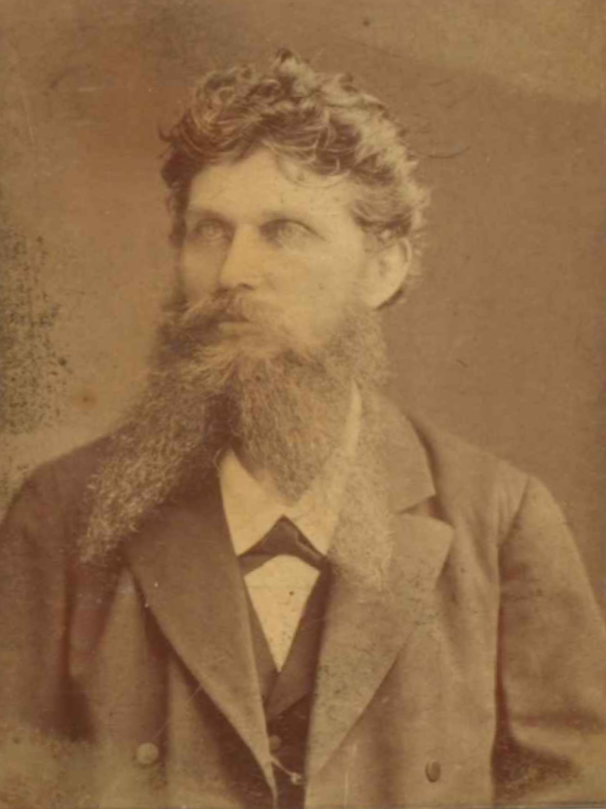
\includegraphics[width=\textwidth, height=\textheight, keepaspectratio]{117-a-slavista_f_x_prusik}
\caption{Český slavista F. X. Prusík (1845 – 1905)}
\label{fig:117-a-slavista_f_x_prusik}
\end{figure}

\begin{figure}
\centering
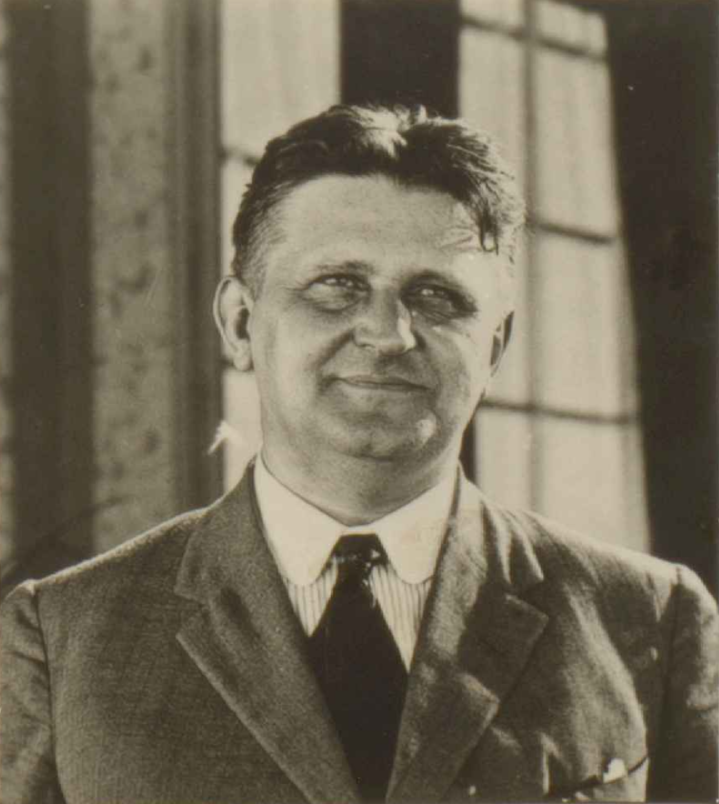
\includegraphics[width=\textwidth, height=\textheight, keepaspectratio]{117-b-prekladatel_dr_borivoj_prusik}
\caption{Překladatel Dr. Bořivoj Prusík (1872 – 1928)}
\label{fig:117-b-prekladatel_dr_borivoj_prusik}
\end{figure}


% str 100 @ 118
V Plzni poznal F. X. Prusík svou budoucí ženu. Byla to Ludmila Šteffelová nar. 25. 8. 1852. Ludmila byla velmi průbojnou ženou a pomáhala svému muži vydatně v jeho práci, naučila se několika jazykům, překládala z nich a o svých častých cestách do ciziny zanechala pozoruhodné paměti. Přežila svého muže o 20 let a zemřela u své dcery Olgy v Jičíně 1. 11. 1925. Svatbu měli 8. 1. 1872 v Plzni.

Z Plzně odešel F. X. Prusík do Příbrami, kde vyučoval až do roku 1877. Tehdy byl zvolen roudnickou obcí za ředitele nově tam založeného reálného gymnasia. O rozkvět mladého ústavu v Roudnici nad Labem staral se až do roku 1885, kdy se zřekl ředitelského místa a odešel do Prahy za profesora na akademické gymnasium. V těch letech byl pak nejagilnějším a jeho život z vědecké stránky byl tehdy nejplodnější.

F. X. Prusík zúčastnil se bojů o pravost Rukopisů. I když později byl Rukopis Královédvorský a Zelenohorský pro­hlášen za padělek, přece jen pro náš národ znamenaly mnoho. Rukopisy byly podnětem k velkým dílům Smetano­vi, Mánesovi i Myslbekovi. Jakou zuřivostí vyznačoval se tento boj v národě, svědčí o tom historka, kterou zaznamenala Ludmila Prusíková ve svých pamětech. Píše: "Onehdy se dal F. Náprstek (známé Náprstkovo museum) dovézti do Masarykovy vinárny v Pasířské ulici a ptal se: "Jste vy také příbuzný toho darebáka Masaryka?" Vinárník odpověděl, že je jeho bratr a že pan profesor sám sedí za stolem. Náprstek spustil na profesora::"Tak to jste Vy, ten lump, co dělá českému národu takovou ostudu, copak z toho máte?" "Mám z toho sto tisíc," odpoví frivolně Masaryk. Na to mu Náprstek: „Sto tisíc Vám za Vaše lum­párny nikdo nedá, ale hanby z toho máte Vy i národ více než za milion!“

F. X. Prusík byl nadšeným obhájcem těchto starých Rukopisů o jejichž pravosti se ještě v roce 1968 vede zase dis­kuse a podrobují se novému chemickému setření, které kdysi dokazovalo nespornou jejich pravost. Nejkrásnější vydání Rukopisu Královédvorského s ilustracemi Máneso­vými a historickým filologickým výkladem F. A. Prusíka, je pěknou památkou na něj .

Kdysi našel F. X. Prusík v plzeňském museu neznámý ruko­pis Husovy Postilly. Ten pak upravil a vydal v roce 1887 ve Věstníku královské české společnosti nauk. Kronika o Alexandru Velikém byla z nejkrásnějších staročeských básní. První překlad Alexandreidy pořídil před staletími Ulrich z Eschenbachu. Aby se i českému národu usnadnila četba této nádherné památky staročeské roman­tiky, upravil ji F. X. Prusik a výkladem opatřil v roce 1896. lato práce byla vyznamenána carskou akademií nauk v Petrohradě. Za své mimořádné jazykozpytné zásluhy byl F. X. Prusík jmen­ován v roce 1891 členem Královské české společnosti nauk.

Když probojovala Eliška Krásnohorská a řada jiných uvě­domělých českých žen právo na to, aby také české dívky
% str 101 @ 119
měly svou samostatnou střední školu, byl F. X. Prusík spolkem Minerva požádán, aby k provedení tohoto nesnad­ného díla přispěl. Měl již v tom směru mnoho zkušeností, ochotně vyhověl Elišce Krásnohorské, zpracoval Minervě vyučovací osnovu a řídil mladý ústav, který byl toho druhu vůbec prvním ve střední Evropě, od roku 1890 s výjimkou roku 1892, až do roku 1895. Patří tedy F. X. Prusík právem mezi zakladatele našeho dívčího středního školství.

Se svou ženou a často i dětmi cestoval F. X. Prusík hojně po světě. Kromě češtiny a němčiny znal výborně rusky, francouzsky a anglicky. Ze svých cest v Rusku, Rakousko-Uhersku, Německu, Holandsku, Dánsku, Belgii nebo Anglii přivážel vždy velmi mnoho cenného materiálu. Tak na příklad píše o návštěvě Naardenu u hrobu Komenského toto:  "Není možno vylíčiti city naše u prostého pahorku, utvo­řeného z balvanů na paměť našeho velikána. Bylo nám divně u srdce, když jsme zřeli místa kde dokonal šle­chetný život svůj, štvaný učenec. V kasárnách pěchoty ukázali nám sklípek, kde našli jeho kosti . Tam teď důstojníci mají pivo. Jaká to profanace! O Komenském v Holandsku vůbec mluví s velikou úctou a v universitní kni­hovně v Amsterodamu, když slyšeli, že jsme z Prahy, uvítali nás velice přátelsky a snesli vše, co se Komenského týkalo, do archivu, kam jinak nemá nikdo cizí přístup." F. X. Prusík objevil tehdy v Holandsku mnoho zajímavého a dosud neznámého o Janu Amosu Komenském. Do té doby se na příklad nevědělo, že v roce 1662 měl Komenský své knihkupectví v Amsterodamě.

Od roku 1887 až 1899 vydával filologický časopis „Krok“. První časopis s tímto jménem byl založen v roce 1818. Redaktorem byl Jan Svatopluk Presl, jeden ze zakladate­lů Národního musea. Třetím časopisem, který měl podob­nou vážnost a nesl v záhlaví jméno Krok, byl Prusikův časopis. Za dvanáct let jeho existence uveřejněné bylo v něm mnoho cenných pojednání, která ještě dnes mohou býti pramenem nových poznatků filologů a historiků.

F. X. Prusík nebyl ovšem jenom vědcem, byl to živý člověk, rád plaval, provozoval cyklistiku i velehorskou turistiku. Styky jeho s vědci i literáty byly rozsáhlé.

V literárním archivu Památníku národního písemnictví v Praze, uložena je jeho korespondence a objevují se zde  jména, která byla ve své době páteří naší kultury. Jsou to na příklad dopisy Julia Zeyera, Jaroslava Vrchlické­ho, Svatopluka Čecha, J. V. Sládka, Václava Vlčka, Soběsla­va Pinkasa, Adolfa Heyduka, T. G. Masaryka, Ignáta Hermana, je zde i 80 dopisů Elišky Krásnohorské z doby zakládání Minervy, ale i Gabriely Preisové, Zikmunda Wintera, Aloise Jiráska a mnoha jiných.

F. X. Prusík zabýval se také pilné etymologií, rozborem místních jmen a starých nápisů českých. Že urbář Gryepeků z Kaceřova, kteří byli kdysi pány nad našimi předky na Kralovicku, zpřístupnil českým čtenářům, je jeho
% str 102 @ 120
dílem. Bylo by toho příliš mnoho, kdybychom se zmiňovali i o cenné korespondenci F. X. Prusíka, kterou, měl v minulém století s nejslavnějšími slavisty té doby Jagičem a Miklošičem a mnoha jinými vědci ve světě. Nesporně patřil F. X. Prusík mezi významné české filology. V posledních letech svého života výrovský rodák, F. X. Prusík dosti marodil a nebylo mu ani 60 let, když 7. června 1905 zemřel na rakovinu ve Stupčicích u Tábora. F. X. Prusík měl šest dětí a z nich tři dospěly. Nejstarší byl syn Bořivoj, který se narodil 31. 10. 1872 v Příbrami. Byl hlavním bibliotekářem Universitní knihovny v Praze, překladatelem a diplomatickým úředníkem a zemřel 1. 4. 1928 v Praze. Druhá byla dcera Ludmila, na­rozená 21. 5. 1876 v Příbrami. Poprvé provdala se za místodržitelského radu Schmatta, podruhé za hoteliéra Pro­kopa na Špičáku na Šumavě. I ona zemřela poměrně mladá 8. 3. 1928. Třetí byla dcera Olga provdaná Schlindenbuchová. Narodila se 2. 11. 1877, žila se svým mužem ve Vlašimi, Opočně a nejdéle v Jičíně, kde je pochována. Zemřela 30. 8. 1953 v Praze.

Vylíčili jsme zdánlivě dlouze, ale přece jen co nejstručněji zasloužilý život a dílo F. X. Prusíka, člena  našeho starého rodu. Jemu vděčíme neobyčejně za mnohé, co jsme o našem rodu předtím nevěděli a co jen dí­ky jeho badatelství je nám dnes o našich předcích známo. F. X. Prusík je pochován na olšanských hřbitovech v Praze a veliké podivení budí jeho dosti zanedbaný stav, když právě on je také zařazen v seznamu slavných lidí, pochovaných na tomto hřbitově, vyvěšeném u hřbitovního vchodu. Jistě by si zasloužila jeho památka větší úcty.

\subsection{Bořivoj Prusík, průkopník slovanských spisovatelů u nás}

První dítě F. X. Prusíka, syn Bořivoj, narodilo se 31. 10. 1872 v Příbrami. Bořivoj byl prvním vnukem výrovského sedláka Václava Prusíka. Gymnasium začal studovati v Roudnici n/L  a když se jeho otec stal profesorem Akademického gymnasia v Praze, dokončil tam studia. Pak studoval na Filosofické fakultě pražské university a také v Mnichově. Za disertační doktorské téma měl dílo slavného německého dramatika, Lessinga. V květnu 1895 byl promován. V roce 1896 stal se volontérem v Universitní knihovně v Praze, kde rychle postupoval. Od roku 1913 do roku 1919 byl vrchním bibliotekářem. Při převratu státním v roce 1918 byl jedním z místoředitelů této slavné instituce. Bořivoj Prusík propagoval jako první v Čechách nové knihovnické metody tj. desetinné třídění a již v roce 1900 pře­ložil zahraniční knihu Decimální klasifikace. Dnes ve všech velkých knihovnách je tato metoda zavedena.

Od svých mladých let věnoval se studiu cizích jazyků a za­čal sledovati vývoj zahraniční literatury. Zvláště se zajímal o literatury ruské a polské, ale i anglickou, francouzskou a německou. Později se stal proslulým překladatelem.

% str 103 @ 121
Bořivoj Prusík i obě jeho sestry Ludmila a Olga učili se cizím jazykům již od mládí. Jejich otec F. X. Prusík velmi pečlivě o to dbal, a v jeho rodině se každý den mluvilo jiným jazykem. Pěstovala se němčina, ruština, francouzština a angličtina. Tak již od dětství také Bořivoj nabýval velmi dobrých znalostí cizích řečí. Pozdě­ji se naučil ještě polsky a vše to mu bylo k neobyčejné­ ku prospěchu později v jeho životě.

V universitní knihovně, kde působil, měl výborný přehled o všech literárních novinkách světových a mnohé z nich začal překládat. Universitní knihovnu doplnil velmi důkladně literaturami slovanskými, což jistě nebylo tehdy bez významu za germanizačního režimu. Za svého života přeložil přes 150 románů, přes 300 her a napsal přes 500 článků do různých časopisů jako byl Světozor, Zlatá Praha, Česká revue, Květy atd. Početnost tato byla někdy, pokud se týkalo dokonalosti a přesnosti výrazu, na škodu. Přece však zůstává jeho nesmrtelnou zásluhou, že svý­mi prvními překlady a někdy i zdokonalenými druhými překlady uvedl k nám poprvé díla mnohých spisovatelů, 0 nichž se později ukázalo, že patří ke stěžejním sloupům světové literatury. K jeho prvním překladům patří Dickensův Klub Pickwicků, Thomase Manna Buddenbrookové, od Boleslava Prusa Grunwald, W. Reymonta  Chlopi, trilogie Napoleon od Gasiorowskeho a mnoho jiných z angličtiny, němčiny, francouzštiny a polštiny.

Zvláštní jeho překladatelskou kapitolu tvoří ruská lite­ratura. Bořivoj Prusík přeložil Gogolovu Ženitbu a Revisora, Gorkého Měšťáky a Na dně, Dostojevského Raskolnikova, Tolstého Annu Kareninu, Puškinovu Kapitánovu dcerku, a zvláště všechny nejvýznamnější divadelní hry slavného Antona Pavloviče Čechova.

S Čechovem, touto velkou postavou ruského a světového dramatu, pojilo ho upřímné přátelství. Jeho slavná díla jako je Racek, Ivanov, Strýček Váňa, Tři sestry nebo Višňový sad jsou prvními překlady Bořivoje Prusíka, jimiž byl Čechov uveden poprvé na českou scénu. V památníku národního písemnictví na Strahově je uložena celá literární pozůstalost Bořivoje Prusíka, jako již před tím se tak stalo s dílem jeho otce. V Leninově knihovně v Moskvě je uchováno na čtyřicet dopisů Prusíkových A. P. Čechovovi z let 1896 až 1904, kdy slavný ruský dramatik předčasně umírá.

Bořivoj Prusík oznamuje Čechovovi, jaký úspěch měly v Praze nebo v Plzni jeho hry. Z této korespondence lze dobře poznat, jak nebylo vždy snadné umístit před šedesáti lety hry, dnes tak proslaveného autora, na české scéně. Tak na příklad v roce 1898 sděluje Bořivoj Čechovovi, že se mu konečně podařilo umístiti Racka na scénu Švandova divadla. Jinde zase sděluje s jakým neobyčejným úspěchem byl přijat v Praze strýček Váňa.

Bořivoj Prusík nedopisoval si s Čechovem jenom když po­býval v Rusku, ale také když se Čechov léčil ve francouzské Nice. Jindy zase Čechov prosil Prusíka, aby mu zaslal ně­kolik fotografií českých lidí, aby poznal jejich fysiognomii. Jindy se zase obrací Prusík na Čechova o radu, jak by bylo možno uskutečnit turné slavné herečky Hanny Kvapilové po Rusku.

% str 104 @ 122
Na přelomu století byl Bořivoj Prusík považován u nás za nejlepšího znalce poměrů v polském a ruském divadelnictví. V té době obraceli se na něho často Jaroslav Kvapil, ředitel plzeňského divadla Vendelín Budil nebo Laudová-Hořicová a mnoho jiných. Když bylo v roce 1907 založeno Vinohradské divadlo, stal se prvním lektorem Dr. Bořivoj Prusík. Od roku 1910 byl pak jeho nástupcem K. H. Hilar. V roce 1910 byl Bořivoj Prusík také dramaturgem tohoto divadla, po něm pak Hilar a Dr. Karel Čapek. Svými překlady otevřel Bořivoj tehdejší málo informo­vané české společnosti nový pohled na ožehavé sociální poměry. Jeho nesmrtelnou zásluhou zůstane, že do Čech poprvé uvedl nejzávažnější díla Čechovova a Maxima Gor­kého.

Bořivoj Prusík napsal také několik vlastních knih. Jde převážně o povídky sociálního rázu.

Když vznikla Československá republika v r. 1918 opustil Bořivoj své místo v universitní knihovně a vstoupil do diplomatických služeb nového státu, působil stále ve Spojených státech severoamerických, kde byl konsulem v Omaze, St. Louis a naposledy byl jmenován generálním konsulem v New Yorku. Bořivoj byl dvakrát ženat. První jeho manželkou byla Polka Anna roz. Greszynská narozená v Nisku, bývalé Haliči, 20. 9. 1874. Byla také literárně činná pod jménem Dolores Prusíková. Manželství toto bylo v roce 1919 rozvedeno a první žena Bořivojova zemřela 25. 2. 1931 v Sadské. Podruhé vzal si za manželku opět ženu cizí národnosti. Byla to Němka Anna Ecklebenová roz. Winklerová. Pocházela také z Haliče ze Záblatí, kde se narodila 23. 5. 1885. V rodině se jí říkalo Melly. Bořivoj, jak vždy říkal, byl s ní šťasten, ale špatná znalost češtiny její mu působila velké obtíže v jeho diplomatic­kém úřadě. Po několikaletém působení v USA vrátil se Bořivoj Prusík do Prahy, působil pak ještě na minister­stvu zahraničí, ale brzy zemřel. Příčinou jeho smrti byla rakovina, jako u jeho otce Františka. Zemřel 1. 4. 1928. Jeho druhá manželka se znovu provdala a jako Sládková zemřela za čtyři roky po něm sebevraždou 20. 3. 1932. Oba jsou pochováni na Olšanech. Bořivoj Prusík nezanechal po sobě žádných potomků, ale zůstalo po něm dobré dílo.

Druhým dítětem F. X. Prusíka byla dcera Ludmila. Narodila se 21. 5. 1876 v Příbrami. Odtud se brzy stěhovala s ro­diči do Roudnice, kde její otec založil nové gymnasium. Ludmila byla velmi krásnou a inteligentní dívkou. Ušlechtilé rysy její povahy jí neopustily po celý život. Již v mladých letech naučila se velmi dobře německy a francouzsky. Poprvé provdala se z místodržitelského radu Emanuela Schmatta, s nímž žila jeden čas ve Vídni a pak v Praze. Měla s nim dcerku, ale ta zemřela v dětství. Brzy pak také zemřel její manžel a za nějaký čas provda­la se opět bez vědomí své matky, za Jana Prokopa. To byl
% str 105 @ 124
majitel známého hotelu Špičák na Šumavě. Manželství bylo uzavřeno v Káhiře v Egyptě. Ludmila Prokopová byla duší celého podniku na Špičáku a mnoho slavných lidí, kteří trávili odpočinek v klínu šumavských lesů, vděčně na ni vzpomínali, často i v literárních dílech. Ludmila zemřela tragicky otravou po vytržení zubu, poměrně mladá 8. 3. 1928 na Špičáku. Je pochována v Železné Rudě. Měla tři děti. Nejstarší je Ludmila, narozená 30. 9. 1912. Stala se magistrou farmacie a jejím manželem byl také lékárník Just. Manželství však bylo rozvedeno. Bydlí v Praze Vršovicích, tř. SNB 99. Má jedinou dceru Jarmilu Justovou, narozenou 7. 5. 1941. Vystudovala historii a praehistorii a působí dnes v Archeologickém ústa­vu v Praze. Může se vykázati již také některými archeologickými objevy na Poděbradsku.

% str 104+1 @ 123
\begin{figure}
\centering
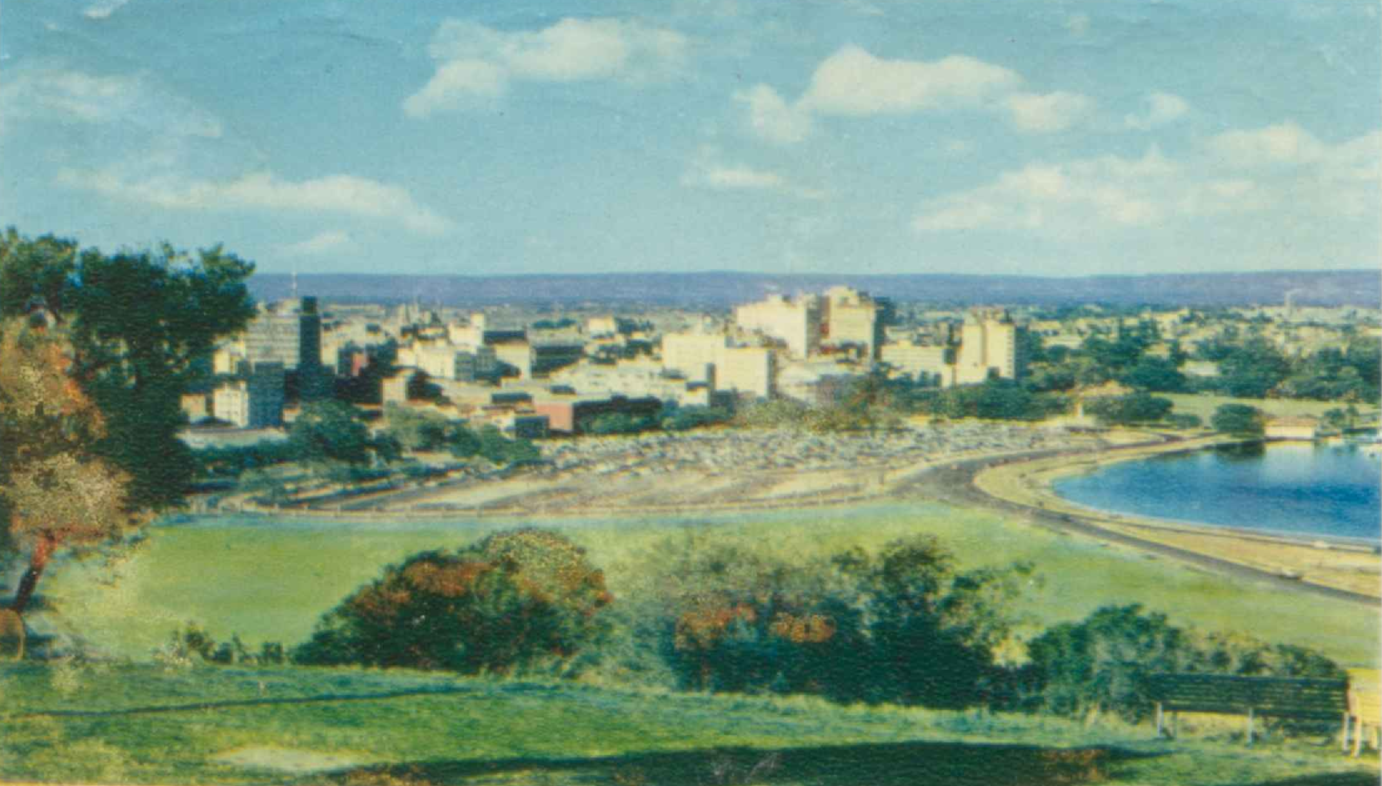
\includegraphics[width=\textwidth, height=\textheight, keepaspectratio]{123-a-mesto_perth}
\caption{V městě Perth v západní Austrálii žije potomek Františka X. Prusíka, Anna Ludikarová}
\label{fig:123-a-mesto_perth}
\end{figure}

\begin{figure}
\centering
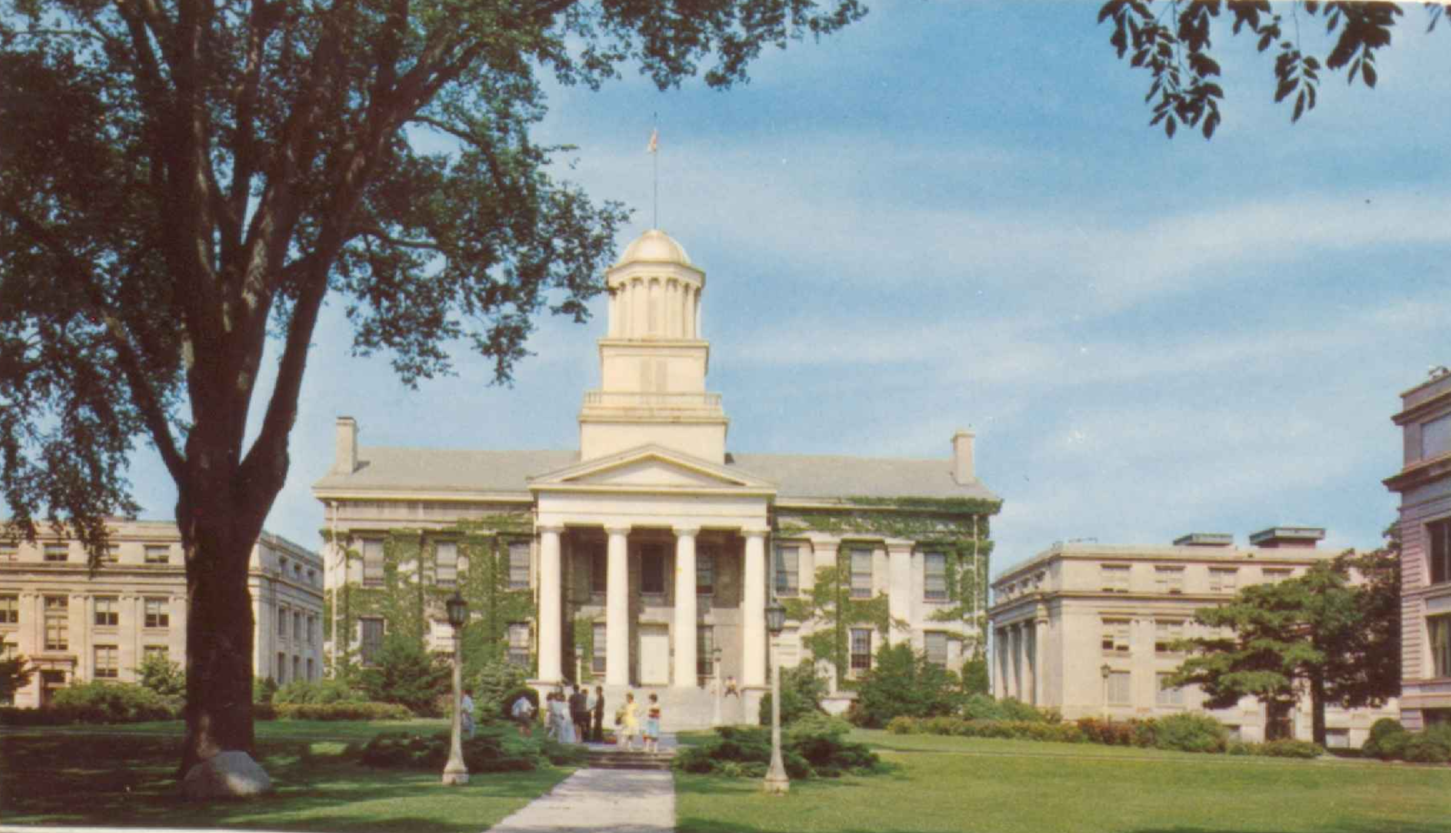
\includegraphics[width=\textwidth, height=\textheight, keepaspectratio]{123-b-iova_city}
\caption{V městě Iova City v USA žijí potomci Marie Prusíkové, provdané Kozové v Potvorově}
\label{fig:123-b-iova_city}
\end{figure}

% str 105 @ 124 (pokr.)
Druhou dcerou je Anna. Narodila se 22. 10. 1914 a je provdaná Ludikarová. V květnu 1949 se vystěhovala z republiky a v září 1950 se dostala do Austrálie. Má dvě dcery. Danica je narozená 14. 1. 1942 a Michaela Ludika­rová je narozena 1. 1. 1948. Dnes mají již všichni australské občanství. Žije v městě Perth na západním pobřeží Austrálie, adresa její je 66, Flinders Street, Tuart Hill. Město, kde dnes Anna Ludikarová s rodinou žije, je rovina, nejsou zde žádné hory, rostou tam palmy, pomeranče, citrony, ale krásné Šumavské lesy kolem Špičáku, kde se narodila, jí tam chybí.

Posledním dítětem Ludmily, Prokopové, roz. Prusíkové, je syn Jan. Narodil se 1. 11. 1915 na Špičáku, odkud po okupaci Sudet musel se svým otcem utéci. Po druhé světové válce se opět ujal řízení hotelu, ale když došlo k znárodnění jeho, působil pak v Praze, Dobříši a zvláště nejdéle v Mariánských Lázních. Zde byl sice považován pro své schopnosti jazykové i organizační za výborného hotelového odborníka, ale jeho činnost pro jeho původ byla mu stále ztěžována. Dnes žije v Mnichově. Dětí nemá. Adresa jeho je: Műnchen, Denninger Strasse, 216.

Posledním dítětem F. X. Prusíka a jeho ženy Ludmily, byla dcera Olga. Narodila se 2. 11. 1877 v Roudnici nad Labem. V roce 1899 provdala se za Hugo Schlindenbucha, který byl správním úředníkem a nakonec vicepresidentem soudu v Jičíně. Žili spolu ve Vlašimi, Opočně a nejdelší čas v Jičíně. U nich také zemřela Ludmila Prusíková, vdova po slavistovi F. X. Prusíkovi. Ta ovšem také časem pobývala u první své dcery provdané Prokopové na Špičáku. Olga Schlindenbuchová měla dva syny. Starší Vladimír je narozený 11. 5. 1901 ve Vlašimi. Stal se komerčním inže­nýrem a působil v Národní bance řadu let a později ve Státní bance. Bydlí v Praze 5, Košíře, Na Výšině 20. Má tři děti. Jiřina, provdaná Kolavíková nar. 7. 4. 1928 bydlí v Praze - Malešicích, Malešická 397. Má dcerku Evu, nar. 12. 5. 1955. Syn Vladimír Schlindenbuch je narozen 19. 12. 1931, je konstruktérem a bydlí v Praze - Hradčanech, Bašta sv. Ludmily č. 3. Má dva synky. Petra nar. 9. 10. 1959 a Michala nar. 13. 4. 1965.

% str 106 @ 125
Druhý syn Vladimíra Schlindenbucha je Svatopluk. Narodil se 12. 2. 1946,  pracoval v jemné mechanice a nyní studuje na technice. Bydlí s rodiči v Košířích. Olga Schlindenbuchová, rozená Prusíková měla druhého syna, který dostal jméno po otci Hugo. Narodil se 11. 6. 1907 v Opočně. Vystudoval techniku a po ukončení studii nastoupil jako měřičský úředník do Nového Města nad Metují. V roce 1935 byl přeložen do Frýdlantu, ale po obsazení Sudet byl pak střídavě v Novém Bydžově a v Jičíně. V roce 1945 vrátil se opět do Frýdlantu jako jeden z prvních Čechů. Tam byl přednostou osidlovací komise min. zemědělství. Dožil se pouze 45 let a zemřel na rakovinu žaludku 17. 11. 1952. Měl tři děti. Syn Jan Schlindenbuch nar. 16. 5. 1943 je dnes horníkem a bydlí ve Rtyni v Podkrkonoší č. 616. Má synka Martina naroze­ného 4. 6. 1966. Druhým dítětem Huga Schlindenbucha je dcera Zuzana, nar. 8. 9. 1946. Je provdaná Bangiová, bydlí nyní v Liberci, Leninova 44. Nejmladší syn Pavel Schlindenbuch, nar. 23. 6. 1949 je vyučeným mechanikem ve Škodovce a žije v Hradci Králové. Tyto tři děti ztratily také záhy i matku a tak jejich život v nejmladších letech nebyl vždy nejsnazší. Předčasná smrt Hugova neobyčejně trápila jeho matku Olgu Schlindenbuchovou. Zemřela za necelý rok po něm v pražské nemocnici 30. 8. 1953.

První dcerou Václava Prusíka a Josefy, roz. Kotasové ve Výrově byla Josefa. Narodila se 28. 2. 1848, tedy několik měsíců před zrušením roboty. Ve svých sedmnácti letech ji provdali za sedláka Matěje Urbánka do Lednice č. 12. V usedlosti, kde pak žila, říkalo se odedávna "u Martinců". Josefě Urbánkové, roz. Prusíkové se zvláště v prvních dobách velmi stýskalo a byla potom neobyčejně šťastná, když v Kozojedech se usadil Václav Prusík z Hodyně. Vedle dvora byl statek Urbánkův největší v obci. Již manžel Josefy byl starostou obce a pak zase její syn František a vnuk Josef. Z manželství vzešlo 12 dětí, ale jen sedm jich dospělo. Josefa Urbánková má nejčetnější potomstvo ze všech dětí Václava Prusíka z Výrova.

Děti, které dospěly, byly: Marie naroz. 24. 9. 1871, provdaná Řezáčová v usedlosti "u Hlušíků" v Lednici, kde zemře­la 10. 4. 1924. Druhá byla Anna nar. 19. 4. 1874, provdaná za hostinského a sedláka Soukupa v Řemešíně, kde zemřela 18. 3. 1953. Třetím dítětem, které dospělo, je František Urbánek, nar. 20. 10. 1876. Ten převzal rodný grunt po ro­dičích a žije u syna a vnuka v Lednici č. 12. Čtvrtá je Kristina nar. 20. 9. 1879, provdala se za Václava Zikmunda v Mladoticích a dnes žije u své vnučky Tůmovcové v České Doubravici. Páté dítě, které dospělo, byl syn Josef. Narodil se 26. 2. 1882. Poměrně dlouho byl doma v Lednici, pomáhal v hospodářství a byl to náruživý muzikant. Pozdě­ji se přiženil do menší usedlosti v Kožlanech, kde zemřel bez vlastních potomků 23. 5. 1946. Dcera Josefa, nar. 5. 10. 1888 provdala se za Františka Sopra, železničáře ve Vroutku,
% str 107 @ 126
kde žije jako vdova. Poslední je Anežka naro­zená 9. 4. 1891. Provdala se za zemědělce Václava Krýsla v Kočíně. Tam dosud žije.

První dítě Josefy Urbánkové roz. Prusíkové z Výrova byla dcera Marie. Narodila se 24. 9. 1871. Provdala se za sedláka Řezáče v Lednici. Byla to neobyčejně dobrosrdečná žena, ale bohužel život její byl poměrně krátký. Zemřela ještě několik dnů před svou matkou a to 10. 4. 1924. Měla čtyři dcery. Anežku, Marii, Annu a Blaženu. Nejstarší Anežka, nar. 20. 5. 1898 byla provdaná Fenclová a zůstala doma. Je to usedlost tak zvaná "u Hlušíků" č. 28. I její sestry Marie a Blažena se provdaly za Fencly, kteří jsou také všichni bratři. Rod Fenclů má dvě zvláštnosti: byli to vždy velcí muzikanti a v jejich rodinách se rodil podivuhodný počet dvojčat. Všichni tito Fenclové vyznačují se velkou inteligencí a láskou k dějinám.

Anežka Fenolová měla tři děti. Dcera Jaroslava nar. 14. 4. 1928 je provdaná Beránková v Rakovníce, Píseckého 768. Každou svou volnou chvíli věnovala vždy svým rodičům a vydatně pomáhala ve svém domově v Lednici. Má tři děti. Josef Beránek nar. 25. 10. 1957, Hana nar. 3. 5. 1961 a Pavel nar. 25. 6. 1963. Pak se Anežce Fenclové narodila 24. 5. 1950 dvojčata, Miroslav a Miroslava. Miroslava je provdaná Lűftnerová v Kralovicích č. 80, má tři děti. Jarmilu nar. 4. 2. 1955, Miroslavu nar. 12. 5. 1959 a Františka nar. 24. 8. 1961. Lűftnerovi pracují v JZD. Miroslav Fencl zůstal doma v Lednici. I on je členem JZD. Má syna Miroslava, nar. 27. 6. 1965, dále Vendulku nar. 12. 10. 1966 a Jaroslava narozeného 1. 5. 1968.  Další dcera Marie Řezáčové, Marie je narozena 28. 3. 1901. Je provdaná Fenclová v Kobčicích č. 2 a má dvě děti. Dcera Jiřina je narozena 7. 3. 1929 a syn Jiří Fencl tentýž den. Zase dvojčata v rodě Fenclů. Jiří je zaměstnán v les­ní správě v Petrohradě a má tři děti. Věra se narodila 28. 9. 1957, Jiřina 8. 8. 1959 a Jiří 26. 12. 1960.

Třetí dcera je Anna, narozená 21. 3. 1904 v Lednici "u Hlušíků“ a provdala se za rolníka Václava Škubala do Dřevce č. 21. Má dvě dcery. Miluše se narodila 24. 8. 1934 a je provdaná zase Fenclová a žije s matkou, v Dřevci. Má dvě děti: Marii nar. 6. 4. 1961 a Václava nar. tentýž den. Již třetí dvojčata. Druhou dcerou Anny Škubalové je Blažena, nar. 18. 9. 1937. Je provdaná Folková v Jarově č. 54 u Plas. Pracují tam také v JZD. Má dvě dcerky, Jiřinu, nar. 24. 2. 1961 a Evu Folkovou nar. 15. 3. 1964.

Nejmladší dcerou Marie Řezáčové byla Blažena. Narodila se 2. 2. 1911 v Lednici a je provdaná Fenclová v Borku č. 2. Její muž byl také jako všichni Fenclové velkým hudebníkem a zahynul tragicky při návratu motocyklem ze zábavy u Liblína. Blažena má dvě děti. Její syn Josef nar. 9. 1. 1939 přiženil se do Žichlic č. 43. Má dcerku Janu Fenclovou nar. 27. 2. 1966 a synka Miloše nar. 26. 12. 1967. Její dcera Blažena je provdaná Tauberová a žije s matkou v Borku. Narodila se 31. 12. 1941 a má synka Zdeňka Taubra, nar. 26. 10. 1966. Anežka Fenclová zemřela 4. 8. 1966. Blažena Tauberová má také dcerku Laděnku nar. 7. 2. 1968.

% str 108 @ 127
Druhým dítětem Josefy Prusíkové provdané Urbánkové v Lednicí byla dcera Anna. Narodila se 19. 4. 1874. Provdala se k Soukupům do Řemešína u Mladotic. Tam měli hostinec a hospodářství. Měla čtyři dcery, Marii, Miladu, Růženu a Annu a syna Josefa. Anna Soukupová zemřela v Řemešíně 18. 3. 1953 .

Nejstarší její dcera Marie narodila se 3. 10. 1903 a provdala se za dělníka Turečka v Chrašťovicích č. 36. Zemřela poměrné brzy jako sedmapadesátiletá 9. 7. 1960. Marie Turečková měla čtyři děti. Stanislav nar. 3. 1. 1932 bydlí v Chrašťovicích a má Stanislava nar. 30. 10. 1961. Ladislav Tureček nar. 23. 5. 1936 bydlí v Dobré č. 69 u Kladna. Pracuje v kladenském průmyslu. Má synka Marti­na nar. 30. 7. 1967. Dcera Marie je provdaná Kočková v Kalci blíže Chrašťovic. Narodila se 16. 7. 1943 a má syn­ka Jaromíra nar. 29. 7. 1967. Posledním dítětem Marie Turečkové je dcera Dana nar. 10. 9. 1953.

Druhým dítětem Anny Soukupové byl syn Josef. Narodil se 5. 8. 1905 v Řemešíně č. 27 a na rodné usedlosti také zůstal. Je dnes členem JZD. Má dvě děti. Dcera Květo­slava je provdaná Hajšmanová a bydlí v Olšanech u Sedlce, kde její manžel je vedoucím farmy státního statku. Květoslava nar. 10. 10. 1935 má dceru opět s tímto jménem nar. 14. 11. 1958. Jejím druhým dítětem je Václav Hajšman nar. 19. 1. 1961. Syn Josefa Soukupa v Řemešíně je také Josef. Narodil se 31. 8. 1941 a pracuje rovněž v JZD. Má dvě děti. Ludmilu nar. 23. 9. 1964 a Vlastimila nar. 30. 3. 1967.

Dalším dítětem Anny Soukupové byla dcera Milada. Narodila se 31. 8. 1907 a provdala se za rolníka Beránka do Borku č. 9. Má jedinou dceru Miladu nar. 20. 10. 1940. Je provdaná Tragenreifová a bydlí v Plzni, Zámečnická 36. Má dvě děti. Dcerka Taťána je narozena 17. 6. 1963 a syn Radek nar. 20. 6. 1967.

Třetí dcerou Anny Soukupové v Řemešíně byla Růžena. Narodila se 26. 1. 1910 a je provdaná Lišková v Řemešíně č. 40. Má tři děti. Její syn Jaroslav Liška nar. 11. 4. 1930 bydlí v Mirošově u Rokycan. Má dva syny, Jarosla­va nar. 10. 9. 1956 a Miroslava nar. 4. 4. 1960. Druhý syn je Miroslav Liška. Narodil se 19. 7. 1931 v Řemešíně a dnes pracuje na Karlovarsku. Bydlí tam v Novém Sedle, Revoluční 194. Má dcerku Miroslavu nar. 28. 6. 1961. Poslední je Josef Liška, nar. 24. 10. 1950 a bydlí se svou matkou v Řemešíně.

Posledním dítětem Anny Soukupové byla dcera Anna. Narodila se 22. 5. 1912 a jako provdaná Jánská bydlí v Řemešíně č. 31. Má dvě děti. Její syn Ladislav Jánský, narozený 17. 4. 1940 má synka Ladislava nar. 10. 9. 1964. Dcera Stanislava provdala se za lesníka Dlouhého. Je narozená 11. 8. 1941 v Řemešíně. Její muž působil urči­tou dobu v polesí Manětín a tam se mu podařilo zastřeliti bílého jelena, což je jistě řídký zjev. Bydleli v Novém Městečku u Nečtin. Dnes bydlí v Bukovině č. 25. Mají synka Milana nar. 7. 6. 1963. Dále se jim narodila 12. 6. 1968 dcerka Stanislava.

% str 109 @ 128
Prvním synem Josefy Prusíkové provdané Urbánkové v Lednici byl František. Narodil se 20. 10. 1876 a převzal doma po rodičích grunt, zv. "u Martinců". Patří dnes k nejstarším členům našeho rodu. Je stále duševně čilý. Dobře si pamatuje ještě svého děda Václava Prusíka ve  Výrově, jemuž pomáhal v menších pracech na statku, kde se narodila jeho matka. Byl to výborný hospodář a ja­ko chovatel koni byl Urbánek proslulý nejen na Kralovicku, ale i v republice. Na výstave koní, na hospo­dářské výstavě v Praze v r. 1929 dostal František Urbánek z Lednice první cenu za vystavovanou klisnu. Urbánkové nebyli nikdy koňskými handlíři jako někteří sedláci, ale opravdovými milovníky chovu koní. František Urbánek byl řadu let starostou Lednice a často zastup0val obec i v Praze, spolu s jinými delegacemi z okresu. Jeho hospodářství je dnes začleněno také do JZD, ovšem jako větší hospodář také si v pohnutých porevolučních dobách musel vytrpěti své. František Urbánek měl dva syny. Za ženu měl Františku, roz. Šourovou z Kozojed. Starší jeho syn je Josef Urbánek, narozený 22. 11. 1904 v Lednici č. 12. Vždy šel v dobré stopě svého otce a když se ten vzdal starostenství, byl i on pro oblibu mezi spoluobčany, zvolen rovněž starostou. Má dva syny. Josef Urbánek nar. 9. 12. 1936 bydlí doma a pracuje v JZD. Má dva chlapce, Luboše nar.  27. 5. 1963 a Václa­va nar. 24. 5. 1965. Jeho bratr Václav Urbánek je na­rozen 30. 12. 1939. Pracuje jako absolvent průmyslovky, jako technik v Kaznějově. Tam má svůj domek. Jeho syn Pavel je narozen 20. 3. 1968.

Druhý syn Františka Urbánka je František. Narodil se 25. 2. 1911 a přiženil se do hospodářství v Lednici, č. 34, kde se říká "u Páterů". Má syna Vladimíra, nar. 5. 6. 1945, který je zemědělským inženýrem. „U Paterů" mívali vždy výborné výsledky v odchovu, prasat. František Urbánek st. zemřel 15. 7. 1968 ve věku 91 a půl roku.

Třetí dcerou Josefy Urbánkové byla Kristina. Narodila se 20. 9. 1879 a provdala se za sedláka Zikmunda do Mladotic. Měla dvě dcery. Marie naroz. 22. 8. 1905 zůstala doma v Mladoticích a provdala se za rolníka ze starého rodu Mixů z Koryt. Zemřela ve svých jednapadesáti letech na rakovinu 11. 2. 1956. Měla jedinou dceru Irenu, nar. 14. 8. 1929. Ta jo provdána za velmi bystrého sedláka Tůmovce v České Doubravici č. 2 u Manětína. Má dcerku Irenu nar. 17. 7. 1954. Kristina žije nyní u této své vnučky v České Doubravici. Druhou její dcerou je Anna nar. 23. 4. 1907. Provdala se za zemědělce Jaroše do Chockova č. 1 u Radnic. Má syna Václava nar. 16. 6. 1935. Je zemědělským inženýrem. Ten má synka Milana, nar. 22. 11. 1963.

Další dcerou Josefy Urbánkové byla Josefa. Narodila se 5. 10. 1888 a provdala se za zaměstnance drah Sopra ve Vroutku. Za okupace žila v Mladoticích. Nyní bydlí u své dcery ve Vroutku, Nádražní 426. Josefa Soprová má dvě děti. Dcera Anna nar. 23. 7. 1919 je provdaná Baláková ve Vroutku. Má čtyři děti. Její dcera Ludmila nar. 29. 4. 1943
% str 110 @ 129
bydlí v Podbořanech, Dělnická 328. Má synka Zdeňka Takáče, nar. 31. 1. 1966. Druhá dcerka Anny Balákové je Jaroslava nar. 14. 11. 1946. Jako provdaná Koderová bydli ve Vroutku, Vidhostická ulice 426. Dále jsou dva chlapci, Josef Balák nar. 15. 1. 1949 a Jiří Balák nar. 21. 11. 1951.

Syn Josefy Soprové Václav, narodil se 13. 6. 1922, pra­cuje a bydlí v Mladoticích č. 94. Má tři děti. Věra Soprova nar. 23. 3. 1950, Václav nar. 4. 9. 1951 a Hana nar. 24. 4. 1955.

Posledním dítětem Josefy Urbánkové z Lednice byla dcera Anežka. Narodila se 9. 4. 1891 a provdala se za zemědělce Krýsla v Kočíně č. 17. Není to daleko od Lednice a ona také nezapomíná na svoje rodiště a nejčastěji ze všech svých sourozenců je vždy navštěvova­la. Má jediného syna Jaroslava. Narodil se 29. 11. 1920, pracuje v JZD a bydlí v Kočíně s matkou a svou rodi­nou. Má dvě děti. Anna Krýslová je narozena 13. 11. 1949 a Jaroslav je narozen 28. 11. 1953. Dále má Anežka Krýslová dvě dcery. Zdeňka je narozena 29. 9. 1922, je provdaná Baborová v Bílově č. 16. Má tři děti. Josefa nar. 6. 9. 1944, dceru Zdeňku nar. 23. 11. 1945 a Jaroslavu nar. 25. 10. 1951. Zdeňka je provd. Houdková v Kralovicích. Druhou dcerou Anežky Krýslové je Blažena. Narodila se 7. 10. 1925 a je provdaná Valentová ve Výrově č. 17. Má syna Jiřího a dceru Marii, ale ty uvedeme blíže pod potomky Veroniky Prusíkové, provdané Valentové, která patří rovněž do odnože Výrov II.

Dalším dítětem Václava Prusíka z Výrova byla dcera Marie. Narodila se 29. 7. 1851 ve Výrové č. 18, provdala se 16. 9. 1873 za sedláka Josefa Koukla v Bílově. Od pradávna říká se tomuto gruntu "u Kymlů“. Marie Kouklová měla čtyři syny. Mikuláše, Františka, Blažeje a Josefa. O nich budeme však vyprávěti podrobněji u větve Sedlec, v odnoži tzv. Bílov, jejíž zakladatelskou byla Kateřina Prusíková ze Sedlce provdaná Kouklová v Bílově. Marie zemřela poměrně mladá, 6. 2. 1908.

Třetím synem, který se narodil manželům Prusíkovým "u Boudů" ve Výrově, byl Václav. Narodil se 2. 1. 1854, odešel jako předtím již jeho dva bratři, Blažej a František, také na studie do Prahy. I o něj v Praze pe­čoval dobrodinec našeho rodu vikář Blažej Prusík. Václav vystudoval v Praze práva, ale doktorského titu­lu nezískal. Stal se magistrátním úředníkem a naposled byl přednostou živnostenského referátu u pražské obce. Zůstal svobodný, žil až do smrti svého strýce Blažeje ve Vikářské ulici na Hradčanech a teprve pak se odstě­hoval dolů do Prahy. Bydlel pak na různých místech, naposled na Vyšehradě. Zde zemřel ve věku 61 let na zápal plic 16. 9. 1915. Jako starý mládenec měl řadu přátel, zvláště dramaturga Františka Stroupežnického. Všechny krásné památky po svém strýci zdědil on a po něm zmize­ly nenávratně v majetku jeho poslední hospodyně.

% str 111 @ 130
Čtvrtým synem Václava Prusíka ve Výrově byl Vojtěch. Dostal jméno po svém dědovi rychtáři výrovském, který sem přišel v roce 1803 ze Sedlce. Vojtěch Prusík narodil se 3. 4. 1856 ve Výrově. Studoval krátce na gymnasiu v Klatovech, ale z těchto studií se brzy vrátil domů a bylo rozhodnuto, že se stane dědicem gruntu. Oženil se s Josefou Julusovou ze Sedlce, narozenou tam 24. 3. 1861. Statek, odkud ona pocházela, stojí naproti gruntu Prusíků, kde stávala již v XVI. století kolébka našeho rodu. Vojtěch Prusík převzal rodný statek ve Výrově 22. 2. 1884. Byl to velký silný a zdravý člověk, a přitom dobrák od kosti. Až do dne, kdy prodal used­lost ve Výrově, byl starostou obce. Od roku 1901 do roku 1905 byl také okresním starostou Kralovicka. Pak ještě do roku 1914 působil jako člen okresního výboru. Když starostoval v Kralovicích, byli tehdy členy okres­ního výboru tito občané z Kralovicka: Josef Holeček z Plas, Antonín Jelínek z Bučku, František Juha z Bílova, Josef Kožíšek z Jarova, František Slach z Kralovic a František Vodák z Dřevce.

Vojtěch Prusík, jako okresní starosta projevil velkou iniciativu. Za jeho éry postavila se silnice Sedlec-Bílov-Potvorov, dále Čistá-Zdeslav, pak Chříč-Studená-Hlince, dále Slatina-Lhota a silnice Mladotice-Křečov. Postavila se škola v Žebnici a v Hedčanech, a byly prováděny velké vodní úpravy na Střele a Mži. Z podnětu Vojtěcha Prusíka byla zahájena akce ke sbír­ce na stavbu Národního divadla v Brně a projeven veřej­ný souhlas s prohlášením města Prahy, týkající se zří­zení slovanských universit v Brně, Lvově a Lublani.

V den svátku Mistra Jana Husa roku 1903 vedl Vojtěch Prusík z Kralovic delegaci ke slavnosti položení základ­ního kamene k Husovu pomníku na Staroměstském náměstí. Vojtěch Prusík patřil mezi vynikající zemědělce. Jako první v okrese zavedl nová hnojiva, čímž se v celém kraji značně pozvedla úrodnost polí, vysazoval ovocné stromy, mlátičku a některé jiné stroje měl také jako první v celém okrese. Patřil také mezi zakladatele agrární strany, která jako jediná obhajovala nejlépe zájmy zemědělců. Vojtěch Prusík se svou ženou Josefou měl čtyři děti. Syna Blažeje, dcery Annu a Josefu a posledního Václava, který se po něm měl státi držitelem gruntu. Vojtěch Prusík zúčastnil se jako voják taženi při okupaci Bosny a Hercegoviny v roce 1878. Často a rád vyprávěl o tom, jak jen zázrakem ušel tam smrti. Jeho pohostinná usedlost byla otevřena každému. A dodnes staří pamětnici ve Výrově na něj s úctou vzpomínají.

Již on, ale zvláště pak jeho syn Václav, toužili však po tom, aby měli ještě větší a modernější hospodářství. K lítosti ostatních členů rodu byl 7. dubna 1912 prodán rodný statek ve Výrově a Vojtěch usadil se v nedalekém Černínském dvoře v Přehořově. Tam měli i pěknou cihelnu, ale když se jeho syn Václav oženil, odstěhoval se Vojtěch
% str 112 @ 131
Prusík se svou ženou ke své provdané dceři do Kolešovic. Tam však žil jen dva roky a zemřel na zápal plic ve věku 64 let dne 15. 3. 1920. Jeho žena ho brzy následovala, zemřela 17. 7. 1920.

Sedlákem Vojtěchem Prusíkem a jeho odchodem z Výrova v roce 1912 zaniká náš rod ve Výrově po meči. Byl tam tedy 109 let, což vlastně není dlouhá doba, ale svými činy zapsali se tam Prusíci jistě dobře a je také dosud jich tam vzpomínáno. Nápis na jejich hrobě v Kolešovicích je jisté správný, že zní takto: "Jejich láska, poctivost a život plný práce a obětavosti jsou nejsvětlejší památkou po nich." Ve Výrově žijí dnes Prusíci z jiných rodových větví.

Nejstarším dítětem Vojtěcha Prusíka a jeho ženy roz. Julusové ve Výrově byl syn Blažej. Narodil se 30. 11. 1884 ve Výrově č. 18. Studoval na gymnasiu v Klatovech, kde učil již jeho strýc Blažej a studoval jeho bratranec Bohumil. Spolu tam maturovali v roce 1905 a spolu také odešli na studia lékařská na pražskou universitu. Spolu také promovali v jeden den v roce 1910. Mladý lékař Blažej Prusík odešel pak na zkušenou do nemocnice v Olomouci. Již tam vynikl nejen v interním lékařství, ale i v chirurgii. Když vypukla balkánská válka v roce 1912, ochotně vyhověl volání po vyslání dobrovolných lé­kařů na pomoc slovanským bratřím. Na Moravě poznal také svou budoucí ženu. Byla to Bedřiška Vocílková, dcera lesmistra, nar. 26. 2. 1890 v Hulíně. S tou se pak usadil v roce 1913 jako lékař v Dobříši. Dostal se tam na přímluvu kněžny Coloredo-Mansfeldské, resp. profesora Kukuly. Pak si zavedl vlastní ordinaci a 40 let působil Dr. Blažej Prusík v dobříšském okrese. Léčil všechno a s vel­kým zdarem. Později nabyl i zubařské praxe, takže li­dé z města i celého kraje nacházeli u něj radu ve všech bolestech svého těla. Blažej Prusík patřil k lidem ote­vřeným, snad i někdy trochu drsným, ale neobyčejně upřímným a obětavým. Když viděl, že má před sebou chudého člověka, nikdy od něho nic nevzal. Jeden čas byl také zástupcem nár. socialistické strany na radnici dobříšské. Jeho smrt 9. 2. 1953 byla podnětem k opravdové lítosti nad jeho nenávratným odchodem, kterou projevili všichni lidé v tomto kraji. Ještě dnes vzpomínají tam lidé na jeho "zázračné prášky" i na to jak výborně spravoval zuby. Jeho žena Bedřiška zemřela 14. 5. 1957. Oba jsou pochová­ni na dobříšském hřbitově.

Blažej Prusík měl jediného syna Karla. Narodil se za první světové války 3. 11. 1915. Studoval na gymnasiu v Praze a ve šlépějích svého otce věnoval se také medicí­ně. Studia však dokončil až po druhé světové válce, ne­boť necelý rok před ukončením svých studií lékařských, zavřeli Němci naši universitu. V době druhé světové vál­ky pracoval jako laborant v dobříšském sanatoriu. Také byl ve spojení stejně jako jeho otec s partyzány, kteří tehdy působili v rozsáhlých dobříšských lesích.

% str 113 @ 132
Pěkně na to vzpomíná spisovatel Eduard Valenta ve svém románu "Jdi za zeleným světlem". Po druhé světové válce dokončil Karel Prusík svá medicínská studia a odešel na praxi do Hradce Králové, kde zvláště pracoval u prof. Dr. Lukla. V té době se oženil s Evou Uhrovou, která se narodila 25. 4. 1926 v Berehově, kde její otec tehdy působil jako vojen­ský veterinář. Z Hradce Králové odešel Dr. Karel Pru­sík do psychiatrické léčebny v Dobřanech, kde pobyl řadu let jako internista a měl tam výborné výsledky. Se svou ženou Evou zavedli tam nové ošetřovatelské a rekreační metody pacientů. Jeho touhou bylo však, aby se vrátil do svého rodiště, Dobříše. Tam také nyní působí jako lékař. Bydlí v Dobříši č. 892. Dům s krásnou zahradou, který si vystavěl jeho otec, padl za obět asanace a nové výstavbě v Dobříši. Dr. Karel Prusík má dvě děti. Blanka je narozena 20. 4. 1950 v Hradci Králové a Pavel 17. 8. 1952 v Plzni.

Druhým dítětem Vojtěcha Prusíka ve Výrově byla dcera Anna. Narodila se 8. 6. 1886 a v roce 1908 se provdala za německého sedláka Arnošta Meixnera z Kolešovic. Tehdy tento sňatek vzbudil značnou nevoli v celé rodině Prusíků a osud její opravdu nebyl pak šťastný. Na výslovné přání své matky vzala si sice majetného člověka, ale velmi náruživého Němce. Anna Meixnerová žila pak v Kolešovicích, u ní zemřeli pak její rodiče, ale po roce 1918 zakoupili si pak ještě větší hospodář­ství v Německých Hořovicích. Po čase hospodářství pro­dali, stali se soukromníky v Praze, ale již před dru­hou světovou válkou měli zase svůj zemědělský podnik. Hospodařili v Chotči u Radotína. Z tohoto manželství narodil se syn Arnošt. I když byl manžel Anny přesvěd­čeným Němcem, přece jen byl k Čechům spravedlivý a Anna s ním, nezasloužili si osudu, který jim připravil květnový převrat roku 1945. Je zajímavé, že ve svém hospodářství ukrývali po nějakou dobu člověka, jehož čin vzbudil v protektorátě velkou sensaci. Byl to Jan Smudek, který zastřelil německého policistu v Kladně. Později podařilo se dostati Jana Smudka do bezpečí v cizině. To jisté nesvědčilo o nenáviděném postoji Arnošta Meixnera k českému národu. V květnových dnech 1945 uká­zal se znovu ve špatném světle nezdravý rys české pova­hy. Meixnerovi byli vyhnáni ze své usedlosti, zajiště­ni a všechen jejich majetek byl rozkraden. Manžel Anny se oběsil a ona se stala úplnou žebračkou. Žila pak stří­davě u svého bratra v Dobříši, v Praze jako služebná a nakonec se usadila se svým synem ve Šluknově. Zemřela 13. 11. 1967 v domově důchodců po krátké těžké nemoci v Krásné Lípě. Ona je posledním člověkem, který se naro­dil na gruntu "u Boudů" ve Výrově a odešel na věčnost.

Její syn Arnošt narodil se 18. 5. 1909 v Kolešovicích. Myslelo se vždy, že převezme tam statek po svých rodi­čích, ale hra osudu byla jiná. Měl různá zaměstnání a nyní je skladníkem ve Šluknově, kde bydlí v Gottwaldo­vě ulici č. 301. Po krátkém, rozvedeném a bezdětném
% str 114 @ 133
manželství žije tam nyní samoten ve vzpomínkách na pohnutou minulost svých rodičů a zvláště na svou milovanou matku. Zůstane vždy ke cti Anny Meixnerové, roz. Prusíkové, že její syn se neodrodil a je Čechem.

Třetím dítětem Vojtěchovým byla dcerka Josefa. Narodila se 17. 3. 1888. Byla to neobyčejné hezká holčička a výborné se učila. Bohužel záškrt, který v minulém století byl tak zhoubný, zkosil její život v deseti letech 26. 5. 1898.

Po Pepičce narodil se syn Václav. Bylo to 2. 3. 1890 a on byl předurčen jako budoucí hospodář. Od svého mládí miloval stroje. Zajímal se zvláště o všechno, co mohlo usnadniti těžkou práci v zemědělství. Vyučil se strojníkem a s mlátičkou, kterou měli ve Výrově jako první v okrese, pomáhal pak při výmlatu v četných okol­ních obcích. Jeho duch byl velmi neklidný a stále směřoval jen k vyšším metám. Byl to Václav Prusík, který přesvědčil svého otce, že grunt ve Výrově je pro ně již příliš malý, pole že nejsou ve velkých kusech zcelena a proto také mechanizace nemůže se tam tak zdárně uplatnit. Uvítal proto rozhodnutí svého otce Vojtěcha, aby se odstěhovali na větší dvůr do Přehořova. Po pře­vratu 1918 se Václav oženil s Marií Řepíkovou z Milostína. Narodila se tam v pěkném statku 1. 1. 1895 a dnes tam ještě jako vdova žije. Po smrti svých rodiči v roce 1920 odstěhoval se Václav do Milostína. Přehořov zdál se mu již zase malý jako před tím Výrov a pak ani v Milostíně, ležícím v bohaté chmelařské oblasti, nebyl příliš spokojen. Podařilo se mu získati velký statek v německé obci Bitozeves u Postoloprt. Zde také jsou rozsáhlé chmelnice. Václav Prusík neobyčejně zmodernisoval své hospodářství v Bitozevsi a mezi německými sedláky byl velmi oblíben. Nikdy však svou národnost nezradil. Když na příklad vtáhla v říjnu 1938 německá vojska do Bitozevse, byl jeho statek jediným, kde nevlál hakenkreuz. A bylo zajímavé, jak se němečtí spoluobčané postavili na jeho obhajobu, když velitel německého vojska toto po­čínání u starosty ostře kritisoval.

Václav Prusík jako velký milovník mechanisace pořídil si s obětmi zadešťování chmelnic a v jednom kritickém suchém roce vyhrál tím vše. Téměř všude byla tehdy v okolí nízká úroda chmele, jen on vykázal hojnou úrodu. Vysoká cena, která se pak platila za chmel, zaplatila mu nákladnou investici umělého zadešťování. Dlouho však v Bitozevsi za okupace nezůstal, neboť jeho dvůr byl nakonec říšskými úřady převzat. Odstěhoval se opět do Milostína kde žil jako soukromník, neboť mezitím hospo­dářství své tam pronajal. Napsal tam v té době zajímavou kroniku své rodiny a zvláště svého života. Po květnu 1945 byl zaměstnán ve státní traktorové stanici a zemřel po­měrně brzy, 14. srpna 1952 v Praze. Příčinou byla otrava po hnisavé angíně.

Václav Prusík měl dva syny, Václava a Bořivoje.

% str 115 @ 134
První syn Václava Prusíka narodil se 27. 8. 1919 v Přehořově. Dostal po otci jméno Václav. Otec jeho, jako podporovatel všeho moderního a průbojného, dal ho na studie na školách Tomáše Bati ve Zlíně. Po návratu ze Zlína hospodařil s otcem, ale všechny plány, které míval on i jeho otec, se zhatily po květnu 1945. V zemědělství pak již nepůsobil, neboť se obával a to prá­vem, že by jako syn kulaka byl i při své nejlepší a nejpoctivější práci vždy obviňován, když by se snad někdy něco nepodařilo. V Karlových Varech jezdil se sanitkou, pak se stal zaměstnancem Jáchymovských dolů a usadil se v Horním Slavkově u Karl. Varů. Bydlí tam v ulici ČSSP č. 3. Oženil se s Blankou roz. Moukovou z Tišnova na Moravě 11. 2. 1925. Mají Spolu dva synky. Václav je narozen 25. 8. 1954 a Bohdan, jemuž říkají Dan, je narozen 26. 10. 1956. Václav Prusík po zrušení Jáchy­movských dolů pracuje nyní v místním průmyslu v Horním Slavkově. Místo velkostatku je tedy jeho místo u soustruhu. Baťovská škola však mu dala to nejlepší pro život. Je úspěšný i zde. On i jeho bratr Bořivoj hrdě se hlásí k našemu rodu a ve všem, co bylo v jejich silách, pomáhali ke zdaru tohoto historického díla. Celá rodina usadila se v srpnu 1968 v Dietlingen (Őstliche 44) u Pforzheimu v Badensku v NSR.

Druhý syn Václava Prusíka a Marie je Bořivoj. Narodil se 8. srpna 1925 v Milostíně. Studoval na zemědělské škole v Roudnici, pak byl zaměstnán nějaký čas jako agronom. I on, jako syn kulaka, z průhledných důvo­dů raději toto zaměstnání opustil a stal se zaměstnan­cem uhelných dolů v Hrdlovce u Duchcova. Tam se oženil s Lucií Borjanovou, která se narodila 30. 7. 1921 v Hrdlovce. Bydlí tam v Duchcovské ulici č. 63. Bořivoj Pru­sík má dcerku Hanu nar. 18. 9. 1952. Věnuje se studiu zdravotnictví.

Třetí dcerou Václava Prusíka ve Výrově byla Anna. Narodila se 15. 12. 1858. Ve svých 26 letech provdala se za Josefa Kouru v Bílově č. 13. Bylo to 13. 2. 1884. Kourové žijí na tomto gruntě prokazatelné již od roku 1558. U statku je krásná zahrada jako málokde jinde a po zhoub­ném požáru, který v třicátých letech zničil téměř polo­vinu vesnice, mají dnes u Kourů také pěkné budovy. U Kourů nejen za života Anny, ale i pak po celou do­bu hospodaření jejího syna Josefa, byl vždy každý upřímně vítán a zvláště pak členové našeho rodu. Anna Kourová měla čtyři děti. Byly to dcery, Marie, Anna a Růžena a syn Josef. Anna Kourová, roz. Prusíková zemřela v Bílově 14. 12. 1935. .Byla nejhezčí z dcer Václava Prusíka.

První dcerou Anny Kourové roz. Prusíkové byla Marie. Narodila se 16. 6. 1885. Provdala se v r. 1911 ke Slachům v Bílově č. 29. Z této usedlosti již začátkem XVIII. stol. provdala se Anna Slachová za Martina Prusíka v Sedlci a sem zase jindy v tom století se přivdala od Prusíků žena ze Sedlice. Rodina Slachů hlásila se vždy k Prusíkům. Marie Slachová měla tři děti. Nejstarší Marie narodila se 22. 1. 1912, druhá Anna 17. 7. 1913 a syn František 27. 6. 1916.

% str 116 @ 135
Také stavení Slachů padlo v roce 1930 za oběť požáru. Marie Slachová zemřela na rakovinu 20. 9. 1943. Nejstarší dítě Marie Slachové, Marie nar. 22. 1. 1912 je provdaná jako Vopatová v Žebnici č. 42. Pracuje tam v JZD. Má čtyři děti. Její dcera Marie nar. 19. 1. 1936 je provdaná Kočová a bydlí v hezkém domku v Loze č. 21. Má dvě děti. Josef Koča nar. 19. 1. 1959 a Hana nar. 11. 6. 1963 . Syn Václav Vopat je narozen 31. 1. 1938 a pracuje a bydlí v Hrádku u Rokycan č. 105. Má dcerku Soňu nar. 4. 6. 1964. Třetí dítě Marie Vopatové Anna, je narozena 8. 7. 1945 a je provdaná Zemanová. Poslední Božena nar. 17. 3. 1948 je svobodná a žije v Žebnici. Anna Zemanová má synka Pavla narozeného 26. října 1968. Druhé dítě Marie Slachové je Anna. Narodila se 17. 7. 1913, provdala se za Vojtěcha Kůsu zaměstnance drah, který byl až do důchodu náčelníkem stanice v Mladoticích. Anna Kůsová má syna Pavla nar. 15. 1. 1943, který jako průmyslovák je zaměstnán v Keramických závodech v Horní Bříze. U Aničky Kůsové, jak se jí říká, byly vždy dveře jejího příbytku přátelsky otevřeny všem příchozím.

Posledním dítětem Marie Slachové byl syn František. Narodil se 27. 6. 1916 a po rodičích převzal usedlost v Bílově. Jeho žena Marie je rozená Kozová z Bukoviny a je také pokrevným členem našeho rodu. Je to potomek Ka­teřiny Prusíkové ze Sedlice, provdané Kouklové v Bílo­vě. Rodina Slachů je velice početná. Nejstarší jejich dcera Marie je nar. 26. 3. 1941, vždy velice obětavě starala se o své sourozence. Byla opravdu jejich druhou mámou. Jako provdaná Vlková žije dnes v Kozojedech č. 49. Má synka Josefa nar. 20. 7. 1966. Pracuje v JZD. Druhý je Václav Slach nar. 31. 5. 1942 a přiženil se do Odlezel č. 11. Má tam dceru Pavlu nar. 30. 10. 1966. Třetí Jiří Slach nar. 25. 7. 1943 pracuje ve strojírně v Dobříši a bydlí ve Dlouhé Lhotě u Dobříše. Má synka Jiřího nar. 30. 6. 1965. Následují: dcera Jaroslava nyní Jánská, nar. 20. 3. 1947, pak František Slach nar. 15. 2. 1949, dále Anna nar. 21. 9. 1950 a Pavel nar. 16. 3. 1955.

Druhým dítětem Anny Kourové byl syn Josef. Narodil se 6. 2. 1888 v Bílově. Josef Koura byl celou řadu let starostou Bílova. Byl to neobyčejně oblíbený člověk nejen v obci, ale i v širokém okolí. Po květnu 1945 byl také předsedou lidové strany na Kralovicku. Josef Koura patřil vždy mezi ty členy našeho rodu, kteří se navzájem rádi stýkali a podporovali navzájem, kde toho bylo třeba. Oženil se s Marií Valentovou z Borku a s ní měl dvě děti. Syna Vladimíra a dceru Marii. Josef Koura zemřel v Bílově 23. 4. 1964. Pohřeb jeho na hřbitůvek potvorovský byl opravdovou manifestací všeho lidu z kraje.

Syn Josefa Koury Vladimír, narodil se 30. 10. 1921. Vystudoval hospodářskou školu a stal se opravdu výborným zemědělcem. Zvláštních úspěchů se dopracoval on a celé JZD v Bílově v semenářství a šlechtitelství. Vyniká tou­též dobrotou jako jeho otec. Má dvě děti.Vladimír nar. 24. 7. 1963 a Marie nar. 28. 5. 1905.

% str 117 @ 136
Druhým dítětem Josefa Koury z Bílova byla dcera Marie. Narodila se 9. 10. 1928, provdala se za úředníka Jílka a bydlí nyní ve své vilce v Žíhli č. 253. Má synka Václava, nar. 14. 11. 1953.

Druhou dcerou Anny Kourové roz. Prusíkové byla Anna. Narodila se 24. 6. 1891 v Bílově č. 13 a byla později provdaná jako Švarcová v Hrádecku č. 37. Její muž tam byl cestářem a měli menší hospodářství. Anna Švarcova zemřela v Hrádecku 25. 2. 1952. Měla jediného syna. Je to Jaroslav Švarc nar. 20. 5. 1920. Je usazen v Hrádecku, je členem JZD, oženil se s vdovou s jedním děckem, ze svého manželství má jednoho syna Vladimíra Švarce, nar. 11. 2. 1948.

Posledním dítětem Anny Kourové z Bílova, byla Růžena. Narodila se 11. 2. 1894 a provdala se za zaměstnance drah Hergeta v Plzni. Bydleli tam dlouho Na Koterově a z je­jich manželství narodily se dvě děti. První byla dcera Anna, nar. 2. 11. 1921. Má dva syny, Petra nar. 13. 3. 1943 a Pavla Švika nar. 9. 2. 1946. Bydlí v Plzni, Plzenecká 23.

Druhým dítětem Růženy Hergetové byl syn František. Narodil se 21. 10. 1923, je ekonomickým úředníkem a bydlí v Plzni, Sušická 38. Má dvě děti. Hanu nar. 3. 12. 1953 a syna Jana nar. 5. 7. 1957. Růžena Hergetová zemřela v Žebnici u Vopatů náhle dne 20. 5. 1958.

Osmým dítětem Václava Prusíka ve Výrově byla dcera Veronika. Své jméno dostala po své tetě, která tehdy žila v Kostelci nad Mží. Veronika Prusíková narodila se „u Boudů" ve Výrově 24. 11. 1861. Ze všech dětí Václava Prusíka a jeho ženy rozené Kotasové zůstala ve Výrově pouze Veronika. Protože ve Výrově z potomků Václavových nežije již žádný Prusík, jsou potomci Veroniky Valentové, jak se provdala 24. 11. 1885, jedinými zástupci po přeslici tohoto rodu usazeného roku 1803 ve Výrově. Od roku 1912, kdy byla usedlost "u Boudů" prodána, směřovaly kroky členů našeho rodu do čísla 20 k Valentům ve Výrově. Všichni bývali vždy vřele přijati. A tato tradice až dosud trvá. Veronika Valentová vždy přepečlivá Hospodyně, na sklonku života sehnuta až téměř k zemi, zemřela ve Výrově 5. 11. 1936 a byla pohřbena v Kralovicích, jako vždy všichni občané z Výrova. Veronika Valentová měla mnoho dětí, ale jen tři z nich dospěly. Byli to synové Vojtěch a Josef a dcera Božena.

Prvním synem Veroniky Valentové roz. Prusíkové, byl syn Vojtěch. Narodil se 26. 5. 1884, tedy ještě půl roku před tím, než se jeho matka provdala za Josefa Valentu. O něm bylo rozhodnuto, že doma nezůstane, ale grunt že dostane mladší bratr. Vojtěch Valenta přiženil se do usedlosti "u Bláhů" ve Výrově a měl tři děti. Zemřel 28. 8. 1945.  Nejstarší jeho dítě je syn Vojtěch. Narodil se 22. 5. 1916 ve Výrově č. 17 "u Bláhů". Byl dvakrát ženat, ale jen
% str 118 @ 137
z druhého manželství má děti. Shodou okolností je druhá jeho žena Blažena také pokrevním členem naše­ho rodu. Oba pracují v JZD ve Výrově. Mají syna Jiřího Valentu nar. 11. 5. 1948 a dceru Marii nar. 26. 10. 1953. I u nich, jako u většiny zemědělců je dnes jejich renovované stavení k nepoznání od dřívějška. Druhým dítětem Vojtěcha Valenty byla dcera Blažena. Narodila se 25. 12. 1918 ve Výrově a provdala se za majitele hostince Šebka v Kralovicích. Tento hostinec je v domě, kde se říká "v zámku". Tento dům, dnes ovšem již změněný, postavil v XVI. století Florian z Gryspachu. Blažena Šebková, jejíž manželství mělo pohnutý osud, má dvě dcery. Václavka se narodila 23. 3. 1945 a je provdaná Jánská a bydlí v Kralovicích č. 184. Má synka Milana nar. 13. 2. 1964. Druhá dcera, Anna Šebková je narozená 22. 7. 1948 a bydlí s matkou v Kralovicích č. 74. -

Druhou dcerou Vojtěcha Valenty ve Výrově je Marie. Narodila se 9. 5. 1920 a je provdaná Chlupová ve Výrově-Hadačce č. 5. Má dvě děti. Pavla nar. 3. 1. 1945 a Marii Chlupovou nar. 25. 12. 1948. Rodina pracuje v JZD.  Pavel Chlup má dceru Janu narozenu 20. 7. 1968.

Druhým synem Veroniky Valentové, roz. Prusíkové byl Josef Valenta, narodil se 18. 2. 1891 ve Výrově. On se stal dědicem gruntu č. 20. Rod Valentů je usazen velmi dlouho, již dávno před tím než přišel do této obce první Prusík ze Sedlce. Josef Valenta, jako již jeho otec, byl výborným hospodářem. Až do posledních chvil svého života pracoval a tak jako mnoho venkovských lidí nebylo ho viděti sedět nečinně. Zvláštních úspěchů, dopracoval se Josef Valenta v chovu prasat a koní. Oženil se s Annou Pirnerovou z Černé Hatě a s ní měl dva syny. Josefa a Vojtěcha. Josef Valenta zemřel v písecké nemoc­nici 9. 6. 1965 a byl pohřben do hrobu svých rodičů v Kralovicích.

První syn, Josef Valenta narodil se 1. 3. 1923. Žije dnes v usedlosti svých rodiči, která svým moderním vybave­ním není k poznání jak vypadalo stavení před požárem v roce 1911, ale ani ještě k poměrné nedávné minulosti. Josef Valenta pracuje se svou rodinou v JZD. Za humny, nedaleko jeho stavení stojí v poli kříž, který postavil 1831 rychtář Vojtěch Prusík. Josef Valenta, potomek tohoto rodu slíbil, že on až do smrti a pak i jeho po­tomci budou vždy pečovati o tuto rodinnou památku. Josef Valenta má dva synky. Josef se narodil 11. 1. 1951 a pracuje ve Škodovce v Plzni, Milan Valenta je narozený 12. 7. 1952.

Druhým synem Josefa Valenty a Anny Pirnerové, je Vojtěch. Narodil se 28. 6. 1928. Po studiu na hospodářské škole absolvoval vysokou školu hospodářskou v Brně a pracuje dnes jako zemědělský inženýr, jako náměstek ředitele státního statku v Kralovicích. Bydlí tam v ulici B. Smetany č. 448. Má dvě dcery. Marie Valentová nar. 23. 3. 1952 a Stanislava nar. 11. 10. 1958.

% str 119 @ 138
Posledním dítětem Veroniky Valentové roz. Prusíkové ve Výrově byla dcera Božena. Narodila se 19. 7. 1897 a provdala se v únoru 1921 za člena našeho rodu, po­tomka výrovského rodáka Tomáše Prusíka, sedláka Ladislava Prusíka v Horní Bříze č. 26. Božena Prusíková, která tam žije, měla dvě děti. Elišku provdanou Noskovou a Ladislava Prusíka, který je zemědělským inženýrem. O nich jsme již vyprávěli v kapitole o odnoži "Horní Bříza III -" jejímž zakladatelem byl druhý syn výrovského rychtáře Vojtěcha Prusíka, Tomáš.

Dalším dítětem Václava Prusíka a Josefy roz. Kotasové ve Výrově, byl syn Josef. Narodil se 27. 2. 1863. Když mu bylo čtrnáct let, zemřela mu matka. Nějaký čas byl u svého bratra Františka Xavera Prusíka, který již jako ženatý, byl profesorem v Příbrami. Když se Josef Prusík dostal pak na studie do Klatov, měl ho tam zase na starosti jeho bratr Blažej, který byl tam tehdy již pro­fesorem na gymnasiu. Po čtyřletém studiu v Klatovech odešel Josef Prusík do Prahy a zde se zase dostal do péče svého strýce, Blažeje Prusíka, vikáře na Hradčanech. V roce 1882 maturoval na tzv. městské střední škole v Praze  (gymnasium). Po svízelných začátcích byl pak při­jat k finanční stráži, kratší čas byl v Českém Brodě, pak v Benešově nad Ploučnicí a dosti dlouho ve Varnsdorfu. Odtud přešel k celnímu oboru do Prahy. V celnictví pak velmi vynikl. Na počátku tohoto století přeložil se svým kolegou Čermákem celní tarif, do té doby existují­cí jenom v německé řeči. Byla to velmi obtížná práce, ale ulehčila úřadování mnoha dalším generacím celních úředníků. V roce 1913 byl pro horlivější své vlastenectví přeložen dále od Prahy, do Kolína. Tam se stal předno­stou celního úřadu. Ihned po konci první světové války byl povolán vládou republiky do Prahy a zde organizoval důležitou sekci v našem zahraničním obchodě. Působil také v Obchodní a živnostenské komoře, jako první Čech, přednášel celnictví na Vysoké obchodní škole v Praze a nakonec byl vyšším úředníkem Státního úřadu statistické­ho. V této své funkci zajížděl jako odborník i do ciziny.

Josef Prusík měl již od mládí literárního ducha, psal básně, mnoho článků do novin, zvláště o životě Čechů v pohraničí, který dobře poznal za svého tamního působení a v roce 1938 vydal knížku o rodu Prusíků, v níž pojedná­vá zvláště o svém rodišti Výrově a lidech, kteří odtud pocházeli. Josef Prusík se poprvé oženil 4. 6. 1901 s Marií Šálovou. Byla to dcera pokrokového sedláka a starosty okresu kouřimského a města Zásmuk. Narodila se v Zásmukách 30. 10. 1878. Život však neměla dlouhý. Zemřela na souchotiny v první světové válce 24. 8. 1916. Podruhé oženil se Josef Prusík s Františkou Basařovou, roz. Barochovskou 15. 4. 1887. Svatba jejich konala se v Praze 21. 11. 1922, ale manželství toto již bylo bezdětné. Z prvního manžel­ství narodili se dva synové. Vladimír a Jaromír. Josef Prusík zemřel na jaterní chorobu 8. 8. 1940 v Praze.

% str 119+1 @ 139
\begin{figure}
\centering
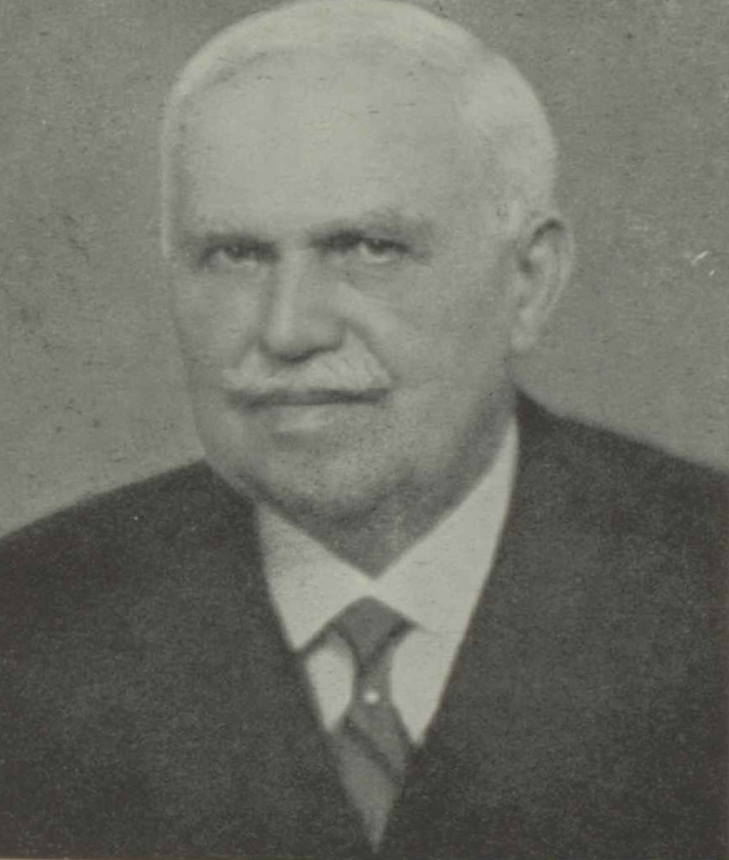
\includegraphics[width=\textwidth, height=\textheight, keepaspectratio]{139-a-josef_prusik_autor_prvni_knizky}
\caption{Josef Prusík, autor první knížky o historii rodu Prusíků, zvláště o rodové větvi Výrov (1863 – 1940)}
\label{fig:139-a-josef_prusik_autor_prvni_knizky}
\end{figure}

\begin{figure}
\centering
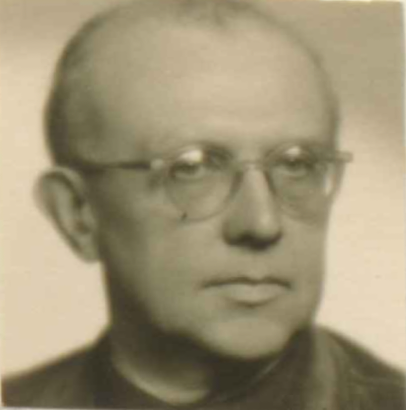
\includegraphics[width=\textwidth, height=\textheight, keepaspectratio]{139-b-autor_jaromir_prusik}
\caption{Jaromír Prusík, autor Dějin rodu Prusíků v celém světě}
\label{fig:139-b-autor_jaromir_prusik}
\end{figure}

% str 120 @ 140
První syn Josefa Prusíka a Marie Šálové je Vladimír. Narodil se v Praze 29. 5. 1902. Studoval na gymnasiu v Kolíně a maturoval v Praze a brzy se pak stal úřed­níkem Městské spořitelny pražské. Zde působil 40 let. Zvláště vynikl v organizačním oddělení tohoto velkého pražského peněžního ústavu. Jeho velikou zálibou je zahrádkářství a to nejen se strany praktické, ale i spolkařské. Všechny své volné chvíle věnoval a věnuje zvele­bení své zahrady v Dobřichovicích č. 426 kde žije. Vladimír Prusík je také veřejně činný v Sokole a MNV v Dobřichovicích. Oženil se s Věnceslavou Landovou, nar. 5. 9. 1910 v Kosoři u Radotína. Její otec byl tam nájem­cem dvora vyšehradské kapituly. Z tohoto manželství narodila se dvojčata, Alena a Jiří dne 8. 12. 1932 v Praze. Vladimír Prusík zemřel náhle 9. 6. 1973 a jeho žena Věnceslava 28. 8. 1972.

Alena Prusíková nar. v Praze byla jeden čas úřednicí v Praze, nyní pracuje v Radotíně. Je provdaná Pechanová, její manžel je vedoucím drogerie v Dobřichovicích. Bydlí se svými rodiči v této obci. Mají dvě děti. Vítězslav Pechan je narozen 13. 7. 1953 a Markéta je narozena 26. 3. 1960. Alena Pechanová zemřela na rakovinu 11. února 1974.

Druhé dvojče, Jiří Prusík vyučil se jemné mechanice. Nyní, jako technik působí u Československého krátkého filmu v Praze. Bydlí také v Dobřichovicích. Poprvé oženil se s Boženou Bojarskou nar. 17. 7. 1932 v Praze. Toto manželství však bylo rozvedeno a Božena Prusíková, podruhé neprovdaná, bydlí v Praze 10, Ulice nad vodovo­dem 487. Z manželství toho narodil se syn Radovan Prusík, 15. 11. 1955 v Praze. Jiří Prusík je podruhé ženatý s Dagmar Svobodovou nar. 5. 10. 1936 v Praze. Radovan Pru­sík bydlí s matkou v Praze, ale o výchovu se stará vydatně jeho otec, u něhož Radovan velmi často v Dobřichovicích pobývá. Z druhého manželství narodila se 12. 7. 1971 dcera Dagmar.

Druhým synem Josefa Prusíka a Marie roz. Šálové je Jaromír Prusík. Narodil se v Praze na Žižkově 13. 1. 1905. Vystudoval gymnasium v Kolíně a v Praze do kvarty a pak studoval na Obchodní akademii v Praze Karlíně, kde maturoval v roce 1924. Po studiích byl dosti dlouho v cizi­ně, zvláště v Anglii a Francii. V roce 1925 stal se odbor­ným redaktorem a ve Vydavatelství odborných časopisu  J. Hložek v Praze zasloužil se o založeni moderního zemědělského týdeníku Hospodářský Obzor. Byl to tehdy časopis, který nejvíce propagoval u nás mechanisaci zemědělství. V roce 1937 vstoupil do podniku republikánské strany Novina a až do května 1945 byl zde činný jako redaktor, zvláště Lidového deníku. Tento list patřil prokazatelně k nejoblíbenějším časopisům na venkově. Po květnových událostech, které změnily značně jeho ži­vot, byl pak jako plánovač ve Svazu pro dobytek, rok byl v Inspektorátu státních statků pro pražský kraj a od roku 1951 do roku 1965 postoupil na pomocného dělníka ve slévárně oceli ČKD v Praze - Vysočanech. Jaromír Prusík napsal v roce 1930 ekonomické dílko ''Konjunktura, krise a budoucnost evropského zemědělství.“

% str 121 @ 141
Podle souhlasné kritiky nebylo do té doby nic podobného u nás napsáno a uveřejněno. - Když ho osud dostal od péra ke kolečku, aby duševně nezakrněl začal se věnovati pátrání po osudech nejen svých před­ků, ale celého rodu Prusíků. Dějiny tohoto rodu jsou jeho dílem. Pokračuje tak ve šlépějích svého otce Josefa Prusíka i jiných členů rodu již dlouho mrtvých. Jaromír Prusík bydlí v Praze 6-Břevnově, Anhaltova 23. Domku, kde bydli na Bílé Hoře v Praze říká se dnes „světo­vé středisko rodu Prusíků".

Jaromír Prusík oženil se 4. 6. 1932 s Jiřinou Eliášovou, dcerou zaměstnance elektr. podniků, která se narodila v Praze 12. 4. 1909. Byla dlouho úřednicí obchodního podniku Řempo. Z tohoto manželství narodil se jediné dítě, syn Zdeněk.

Zdeněk Prusík narodil se 11. 6. 1933 v Praze, vystudoval gymnasium v Praze 7 a pak studoval na matematicko-fysikální fakultě Karlovy university v Praze. Byl promován v červenci 1957 a začal pak hned pracovat jako aspi­rant v Ústavu organické chemie a biochemie ČSAV v Praze Dejvicích. Zde má značné úspěchy a je přednostou odděle­ní, kam se jezdí učit i biochemici a fysikální chemici z mnoha cizích států. Je doktorem přírodních věd (RNDr.) a v roce 1962 byl prohlášen kandidátem chemických věd. Ve své úřední funkci byl již častěji v cizině, kde nejen studoval, ale i přednášel. Oženil se 26. 4. 1958 s Miluškou Ortovou, narozenou 1. 4. 1934 v Praze. Její otec je doktorem práv a působil v Kanceláři presidenta repu­bliky v Praze. Zdeněk se se svou ženou seznámili již ja­ko studenti na universitě, kde jejich společným zájmem byla chemie. I jeho žena pracuje jako chemička ve výzkum­nictví tohoto oboru a to ve Výzkumném ústavu makromole­kulární chemie v Praze 6. Je také doktorkou přírodních věd. Bydlí spolu v Praze 6-Petřiny, Nad Alejí 1766. Z tohoto manželství narodily se dvě dcerky; Hana nar. 24. 6. 1959 a Ivana nar. 25. 2. 1964.

Františka Prusíková, druhá manželka Josefa Prusíka, rodem ze Lštění u Čerčan v Posázaví, zaslouží si ještě mimo­řádné zmínky. Stala se výbornou druhou matkou Vladimíru a Jaromírovi Prusíkovi, kteří tak brzy osiřeli. Ale je známa v našem rodu i jinak. Když v roce 1940 ovdověla, láska a zájem, který věnoval Josef Prusík svému rodu, přešla jako dědictví po něm na ni. Byla vždy neobyčejně obě­tavou pomocnicí všem, kdož ji o to požádali. A to nejen v úzké rodině, ale i všude jinde, kde jí bylo zapotřebí. Mnohokrát vypomáhala v místě, kde žijí nebo žili sourozenci Josefa Prusíka, ať to byl Výrov, Bílov či Lednice. Také často, když byla zavolána, pomáhala řídit domácnost lékaře profesora Prusíka. Neměla svých dětí a proto mateřskou láskou obklopila nejen děti svého muže, ale i vnoučata a pravnoučata.

% str 122 @ 142
Poslední dcerou Václava Prusíka ve Výrově byla Barbora. Narodila se 27. 11. 1865. Jako dvanáctiletá osiřela po matce a život neměla vždy tak snadný. Dokud se nevdala, vypomáhala na různých místech. Dlouho byla u svého bratra Blažeje v Klatovech, několik let také vedla do­mácnost svému příbuznému děkanu Václavu Kouklovi ve Spá­leném Poříčí u Plzně. Sestry i bratři a zvláště otec starali se, aby jejich Baruška netrpěla nouzí a příkoří. Vdala se v roce 1902 za majitele puškařského závo­du Rudolfa Waltera v Klatovech. V té době byl její muž již vdovcem a měl syna Vojtěcha, který také studoval ve stejné třídě na gymnasiu v Klatovech jako byli bratranci Bohumil a Blažej Prusík a Blažej Koukl. Vojtech Walter stal se později ředitelem ve Státním školním na­kladatelství v Praze. V Praze zemřel bezdětný. Ačkoliv nebyl pokrevným členem našeho rodu, vždy se hlásil k němu a také se zúčastnil prvního sjezdu rodu Prusíků, který se konal z popudu Jaromíra Prusíka 26. 10. 1958 v Praze v Obecním domě.

Barbora Walterová roz. Prusíková, či jak se jí v ro­dině říkalo Betty a její klatovský domov, to vše stalo se střediskem celého našeho rodu a zvláště od té doby, co Blažej Prusík, profesor na gymnasiu, odešel do Prahy. Od roku 1905 až do roku 1958 jezdilo se do Klatov k Betty Waltrové. Nebylo to jen na známou klatovskou pouť, ale i bydlívaly i u ní dcery jejích sourozenců a dalších. Prostě, Klatovy a teta Betty staly se útočištěm našeho rodu. Její manžel zemřel v roce 1928 a Betty Walterova ho tedy přežila o 30 let. Zemřela 29. 5. 1958 v Klatovech a ze všech členů rodu se jménem Prusík, či Prusíková, se dožila prozatím nejdelšího věku, téměř 93 let. Byla to předobrá žena.

Posledním dítětem, které se narodilo „u Boudů“ ve Výrově v rodině Václava Prusíka, byl syn Antonín. Narodil se 19. 2. 1869. Když mu bylo osm roků, zemřela mu matka. Studoval několik let na gymnasiu v Klatovech, ale tam se mu příliš nelíbilo. Dostal se pak do státní služby k finanční stráži. Již před tím, jako voják na manévrech v roce 1888 poznal se v Příbrami s Leopoldinou Adamcovou. O této jeho velké lásce a dalším osudu Antonína Prusíka a Leopoldiny nechme vyprávět nevlastni dceru Antonína, Leopoldu Pospíšilovou, žijící v Žamberku. Podobá se to románu.

“Když bylo mamince 17 let, byly v Příbrami a okolí manévry a s nimi tam jako voják přišel i Antonín Prusík. Dům, kde bydlela má matka, sousedil se zahradou, kde byl hostinec a kuželník. Tam se Antonín Prusík seznámil s mou matkou. Měli se hrozné rádi, ale dědeček této známosti nepřál. Zakázal styky jemu s maminkou a ta zdrcená ztracenou láskou, odjela do Vídně. Při loučení jí Prusík řekl: ‚Až něčím budu, slečno Poldi, já si pro Vás přijdu.‘ Léta plynula, a Antonín Prusík se nehlásil. Mezitím se maminka provdala za mého otce, kominického mistra, Karla Pletichu. Byl vdovcem a měl čtyři malé děti. Zemřel po devítiměsíčním
% str 123 @ 143
manželství a já se za deset dní po jeho smrti narodila. Tehdy bylo matce 25 let, byla vdo­vou a matkou pěti dětí. Když se končil rok jejího vdovství, navštívil neočekávaně babičku Antonín Prusík. Byl finančním respicientem a žádal o ruku slečny Poldi. Jak babička vyprávěla, byla přímo omráčená. Řekla mu, že přišel pozdě, Poldi že je již vdovou. Po prvním překvapení prohlásil, že to nevadí a že si ji jako vdovu vezme. Babička ho upozornila, že to nepůjde, že má pět děti. Ani to ho neodstrašilo a dodal, že ty děti také uživí. Jaká to byla láska a charakter! Ale i pak mu babička řekla, že to není možné, protože má maminka výborně zavedenou a skvěle prosperující kominickou živnost a té že se k vůli dětem nemůže vzdát. To ho velmi zarazilo, chvíli mlčel a přemýšlel a nakonec se ptal, zda by ne­mohl tu živnost s ní vést.

Když takto Antonín Prusík s babičkou stále jednali, otevřely se dveře a maminka vešla. Při výkřiku ‚Toníčku‘ omdlela. Vím jen dnes, že Prusík se vyučil za šest týd­nů v Hořovicích kominickému řemeslu a oženil se s mou matkou. Nikdy však nevymetal, měl k tomu pět tovaryšů a několik učedníků. Z tohoto šťastného manželství se narodila dcera Anna, která zemřela v témže týdnu co její otec. Po jeho smrti za šest měsíců se narodil hošíček, Otoušek,  ale i ten do roka zemřel. Po těch­to hrozných ranách se maminka duševně i fysicky zhrou­tila a tu ji pozvaly dvě sestry Prusíkovy k nim na venkov na Kralovicku. Když se však maminka po třetí vdala, tyto styky přestaly. Moje matka prožila pak ještě těžký život. Po třetí si vzala dobrodružného herce, který ji připravil o všechno jmění, dům v Příbrami byl dán do dražby, dědeček s babičkou a ostatní sourozenci s maminkou se rozešli a ona odešla do světa. Byla tedy u divadla a když její muž Kabátník za pět let zemřel, byla již tak vpravená do divadelních poměrů, že si zažádala o koncesi a měla pak na Moravě svou divadelní společnost, pod jménem Jará. Já byla vychována u babič­ky. Po čtvrté vdala se matka za herce Harrera, který byl u ní režisérem. Měla s ním dvě děti, synek zemřel a u mé nevlastní sestry Růženy zemřela pak maminka v Luhu u Příbrami, 15. 1. 1951. Byla narozena 5. 4. 1871 a dožila se téměř 80 let přes tak dramatický život. Když jsem toto jako mladé děvče slýchávala vypravovat, byl pro mne můj nevlastní tatínek Prusík ideálem muže a ctila jsem ho, byť jen ve vzpomínkách, pro jeho ryzí charakter. Má teta, která zemřela v domě důchodců v Žatci, znala ho osobné a ta mně vždy říkala, jaký to byl krásný muž a jaký hodný člověk a jak nesmírně měl maminku rád."

Tak vzpomíná na svou matku a na svého nevlastního otce Antonína Prusíka, Lea Pospíšilová rodačka z Příbrami a žijící dnes pod Orlickými horami v Žamberku. Antonín Prusík byl nejmladší z jedenácti děti, narozených "u Boudů" ve Výrově a zemřel první. Bylo to 13. 4. 1899. Příčinou byl zápal plic. Bylo mu jen třicet let a potom­ci po něm nejsou žádní.

% str 124 @ 144
Vypravovali jsme vám poměrné obsáhleji o potomcích Václava Prusíka z Výrova. Má to několik důvodů. Jednak osudy členů této rodové odnože, nazvané Výrov II, jsou nejlépe známy a dalším důvodem je také, že v dějinách našeho rodu bylo snad v této odnoži nejvíce lidí, kteří se svým dílem proslavili a vynikli nad průměr. Václav Prusík, sedlák a starosta výrovský, nezanechal sice po sobe tolik potomků jako třeba obě jeho sestry, Anna a Rosalie provdané v Horní Bříze, ale přece jen počet je úctyhodný. Nepočítáme-li do souhrnu potomky jeho dcery, provdané Kouklové v Bílově, která je zahr­nuta do větve tzv. Sedlec, zanechal Václav Prusík se svou ženou Josefou 225 potomků, z toho 33 již je mrtvých.

Tato odnož a vůbec celá větev Výrov i sama obec zůstane vždy zvláštním pojmem pro náš rod, i když Sedlec je základním kamenem. Z Výrova však vzešla nejsilnější rodová větev, která také rod Prusíků proslavila.

Výrovská odnož větve Výrov je jasným dokladem, že vývoj dětí je z největší míry závislý na rodičích. Že z této odnože větve Výrov vyniklo nejvíce lidí, bylo i proto, že hlava rodiny byl člověk, který viděl dopředu. Václav Prusík nebyl jen pilným čtenářem, ale i písmákem. Nikde snad v celém rodě Prusíků nebyla vedena tak dlouho a pečlivě rodinná kronika. Sedlák Václav Prusík ji psal sám přes 50 let. Dnes nám představuje výborný přehled o všem, co se v 19. století dělo ve veřejnosti i v rodině, jaké bylo počasí a zkázy. Je to prostě bohatá studnice vědomostí o zašlých časech, z níž zase čerpají další potomci víru a sílu pro budoucnost. Pokračoval v ní syn Vojtěch.

Kdo z vás, z členů veliké rodové větve Výrov, navštíví jednou vesnici Výrov, jistě nezapomene, aby navštívil kapli sv. Vojtěcha, která zde byla vysvěcena 27. dubna 1902. Stojí u zahrady statku č. 18, kle žil zakladatel větve rychtář Vojtěch Prusík, rodák ze Sedlice, a pak jeho potomci. Za hlavního iniciátora je možno považovati Blažeje Prusíka, rodáka výrovského a později profesora gymnasia v Klatovech. Kromě knížete Metternicha, on a jeho bratři se také podíleli největším finančním podílem na vybudování tohoto svatostánku. Kaplička sv. Vojtěcha ve Výrově je krásnou památkou na náš rod. Nechť je po věky zachována v dobrém stavu!
\end{document}
